\documentclass[11pt]{article}
 
\usepackage[T1]{fontenc}
\usepackage[polish]{babel}
\usepackage[utf8]{inputenc}
\usepackage{lmodern}
\usepackage[usenames,dvipsnames]{xcolor}
\usepackage{hyperref}
\usepackage{multirow}
\usepackage{graphicx}
\usepackage{float}
\usepackage{amsmath}
\usepackage{enumerate}
\selectlanguage{polish}
\linespread{1.08}
\usepackage[a4paper, left=2.5cm, right=2.5cm, top=3.5cm, bottom=3.5cm, headsep=1.2cm]{geometry}

\title{\textcolor{BrickRed}{\Huge FAQ W4,\\czyli co każdy student Wydziału Elektroniki powinien wiedzieć}\\}
\author{Rada Starostów Wydziału Elektroniki}
\date{1.02.2021}

\begin{document}
\maketitle

\vspace{0.5cm}

\begin{center}
\fbox{
\includegraphics[scale=1.0]{logo.png}}
\end{center}
\newpage

\tableofcontents

\newpage

\section{Wstęp} 
\indent \hspace{0.5cm} Nie każdy z Nas jest w stanie posiadać wiedzę na każdy temat. Gdy brakuje Nam jej w jakimś zakresie, zwykle zwracamy się z prośbą o pomoc do innych osób. Dlatego postanowiliśmy Wam pomóc, tworząc dokument zawierający wiedzę przydatną podczas całego toku studiów. Mamy nadzieję, iż informacje zawarte w Naszym FAQ ułatwią Wam poruszanie się \linebreak po wszystkich dziedzinach życia uczelnianego, a zdobytą wiedzą podzielicie się z innymi studentami Naszego Wydziału. Powodzenia! \\

\newpage
\section{Informacje ogólne}
\subsection{Mapa kampusu}
\begin{figure}[H]
    \centering
    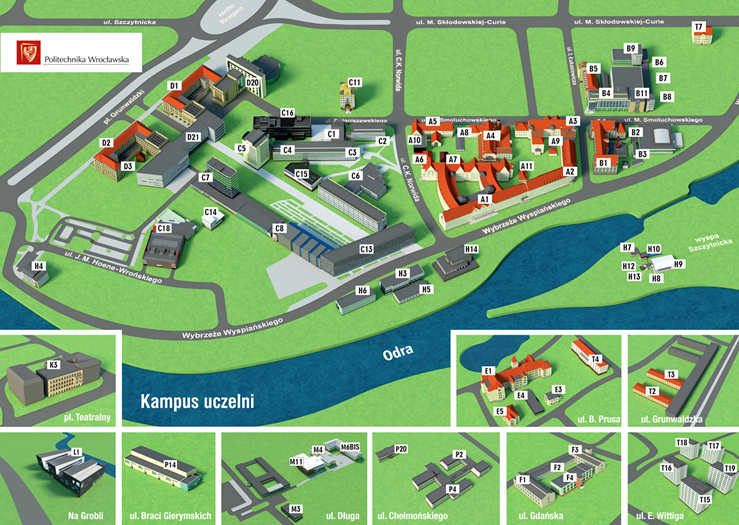
\includegraphics[width=\linewidth]{mapa.png}
\end{figure}

\textbf{Które miejsca na uczelni są ważne, jeśli chcę załatwić jakąś „papierkową robotę” związane ze studiami?}
\begin{itemize}
\item Dziekanat – C-1, s.102 a, na lewo po wejściu głównymi drzwiami
\item Sekcja informatyczna – C-3, s. 12
\item Sekcja dydaktyczna – C-5, s. 109
\item Prodziekani – C-3, s. 13 (lub ich prywatne pokoje, ale najpierw należy napisać maila).
\end{itemize}
\textbf{Czy istnieje mapa rozmieszczenia sal w każdym budynku?}\\
\indent Na aktualną chwilę niestety nie, lecz istnieje aplikacja „PWr Nawigacja” umożliwiająca namierzenie odpowiedniej sali na Naszym kampusie. Aplikacja dostępna do pobrania w sklepie „GooglePlay”.

\newpage
\subsection{Parking na terenie PWr}
\indent \hspace{0.5cm} Na terenie Politechniki do dyspozycji studentów są udostępnione 3 parkingi:
\begin{itemize}
    \item Parking Wrońskiego – 207 dostępnych miejsc parkingowych
    \item Parking przy C-13 (Polinka) – 54 dostępne miejsca parkingowe
    \item Parking przy D20 – 76 dostępnych miejsc parkingowych
\end{itemize}
\indent \hspace{0.5cm} Miejsca parkingowe zapełniają się bardzo szybko, więc aby móc zaparkować na terenie Politechniki należy przyjechać w godzinach porannych (znalezienie wolnego miejsca parkingowego w godzinach 9:00-13:00 graniczy z cudem).\\\\
%Tutaj gdzieś widziałem dokument jakiś w którym był mniej więcej wykaz tego, jak przydzielony jest parking (studenci/pracownicy uczelni)
\textbf{Co zrobić, aby móc zaparkować na terenie Politechniki?}\\
\indent Należy zalogować się na stronie: {\color{blue}\url{http://skd.pwr.edu.pl}} (dane do logowania 
jak do systemu poczty studenckiej), następnie przypisać do swojego konta numer rejestracyjny auta. \linebreak Dane o numerach rejestracyjnych są aktualizowane o wyznaczonej godzinie, więc aby zmienić numer rejestracyjny/przypisać nowy numer rejestracyjny, musimy to zrobić do godziny 23:59, jeśli chcemy zaparkować na terenie Politechniki w następnym dniu.\\
\indent Po przypisaniu numeru rejestracyjnego wystarczy podjechać pod szlaban jednego z wymienionych powyżej parkingów i użyć swojej legitymacji studenckiej, zaczekać do momentu rozpoznania Naszej tablicy rejestracyjnej przez system (system bardzo często nie rozpoznaje tablicy, więc zalecamy użycie legitymacji studenckiej), wjechać na teren parkingu i zająć jedno z wolnych miejsc.\\\\
\textbf{W jakich godzinach samochód może przebywać na terenie parkingu?}\\
\indent Samochód na parkingu może przebywać w godzinach od 6:00 do 22:30.\\\\
\textbf{Czy parkowanie na parkingach PWr jest darmowe?}\\
\indent Tak, parkowanie przez studentów na wyżej wymienionych parkingach 
jest darmowe.\\\\
\textbf{Co zrobić, gdy nie zdążyłem wjechać na parking?}\\
\indent Szlaban wjazdowy/wyjazdowy zamyka się automatycznie po ok. 20 sekundach od momentu poprawnej autoryzacji użytkownika. Jeżeli w tym czasie użytkownik nie wykona wjazdu/wyjazdu z/na parking system mimo wszystko zanotuję tą czynność na podstawie prawidłowej autoryzacji. Zachowanie takie uniemożliwi kolejny wjazd na/wyjazd z parkingu i konieczne będzie skorzystanie z pomocy obsługi parkingu.\\\\
\textbf{Gdzie mogę sprawdzić liczbę wolnych miejsc na parkingach?}\\
\indent Przed wjazdem na dany parking oraz na stronie: {\color{blue}\url{http://iparking.pwr.edu.pl/}} (dostępna jest także aplikacja na telefon).\\\\

\newpage
\section{Dokumenty związane z tokiem studiów}
\subsection{Regulaminy}
\indent \hspace{0.5cm} Od 1 października 2019 roku obowiązuje regulamin studiów wraz z poprawkami znajdujący się na stronie Politechniki Wrocławskiej. Aktualna wersja regulaminu dostępna jest pod adresem:
{\color{blue}\href{https://pwr.edu.pl/studenci/organizacja-nauczania/regulamin-studiow}{REGULAMIN}} \\
\indent Od 31 stycznia 2007 roku obowiązuje następujący Regulamin Wydziału dostępny pod adresem: 
{\color{blue}\href{http://weka.pwr.edu.pl/o-wydziale/o-nas/regulamin-wydzialu}{REGULAMIN-W4}} \\
\indent Studenta PWr obowiązuje także Kodeks Etyki Studenta Politechniki Wrocławskiej dostępny pod adresem:
{\color{blue}\href{https://samorzad.pwr.edu.pl/fcp/8GBUKOQtTKlQhbx08SlkTVgJQX2o8DAoHNiwFE1wZDyEPG1gnBVcoFW8SBDRKTxMKRy0SODwBBAEIMQheCFVAORFCHzY/56/public/kodeks-etyki-studenta-pwr.pdf}{KODEKS-ETYKI}} \\\\
\textbf{Komu mogę zgłosić zachowanie prowadzącego niezgodne z regulaminem?} \\
\indent Na początku najlepiej zgłosić to do Starosty, który zwróci się w Waszym imieniu 
do organów wyżej. Jeśli Starosta nie chce jednak nic zrobić w Waszej sprawie, należy zwrócić się \linebreak do Samorządu Studenckiego Wydziału Elektroniki. Zwrócenie 
się do Dziekana jest ostatecznością i powinien to w Waszym imieniu zrobić przedstawiciel wybrany przez Samorząd Studencki. 

\subsection{Plany i programy studiów}
\indent \hspace{0.5cm} Plany i programy studiów są dostępne do wglądu w dwóch miejscach:
\begin{itemize}
\item na stronie Wydziału Elektroniki: 
{\color{blue}\href{http://weka.pwr.edu.pl/studenci/plany-i-programy-studiow/plany-i-programy-studiow}{PLANY-I-PROGRAMY}}
\item na jednej z podstron portalu EDUKACJA.CL:
\begin{enumerate}
\item Po zalogowaniu się na portal EDUKACJA.CL wybieramy zakładkę „Uczelnia” (prawy górny róg)
\item Następnie wybieramy „Prog. naucz./plan studiów” z „Dostępne opcje” 
(lista z lewej strony)
\item EDUKACJA.CL pokaże przeznaczone dla Nas programy nauczania i plany studiów, ale możemy także przejść w tryb wyszukiwania i wyszukać program nauczania/plan studiów, który Nas interesuje.
\end{enumerate}
\end{itemize}
\indent \hspace{0.5cm} Ponadto, uzupełnieniem planów i programów studiów są karty przedmiotów oraz efekty kształcenia dostępne na stronie Wydziału Elektroniki:
\begin{itemize}
    \item karty przedmiotów:
    {\color{blue}\href{http://weka.pwr.edu.pl/studenci/plany-i-programy-studiow/karty-przedmiotow}{KARTY}}
    \item efekty kształcenia:
    {\color{blue}\href{http://weka.pwr.edu.pl/studenci/plany-i-programy-studiow/efekty-ksztalcenia}{EFEKTY}}
\end{itemize}

\newpage
\section{Organizacja Uczelni i Wydziału}
\subsection{Rektor i Prorektorzy Politechniki Wrocławskiej}
\begin{center}
\fbox{
\includegraphics[scale=0.75]{rektorzyipro.PNG}}
\end{center}

\subsection{Dziekan i Prodziekani Wydziału Elektroniki}
\begin{center}
\fbox{
\includegraphics[scale=1.8]{dziekani.png} }
\end{center}



\newpage
\subsection{Sekcja informatyczna}
\indent \hspace{0.5cm} Jeśli twoje konto na EDUKACJA.CL/JSOS/Serwerze pocztowym nie działa, bądź na tych portalach pojawiają się jakieś błędy, należy zwrócić się do sekcji informatycznej.\\
\indent Wszystkie aktualne informacje o godzinach przyjęć oraz o kontakcie z sekcją dostępne są \linebreak na stronie:
{\color{blue}\href{http://weka.pwr.edu.pl/o-wydziale/kontakt/sekcja-informatyczna}{SEKCJA-INF}}.\\\\
\textbf{Czy jeśli nie dostałem natychmiastowej odpowiedzi od sekcji, mój mail do nich dotarł?}\\
\indent Tak, mają zbyt dużo pracy, by odpisywać szybko na maile. Zwłaszcza w trakcie okresu zapisów (multum maili i telefonów jednocześnie). Pisząc maila pisz konkretnie. W temacie napisz zwięźle o co chodzi: 'zapis ponad stan', 'zapis administracyjny', 
'prawo do zapisów', 'kursy zamienne', etc. Nie wysyłaj tej samej wiadomości kilka razy. W treści wymień kilka opcji, uwzględniając, że coś może się zmienić. Upewnij się, 
że wysłałeś wiadomość na dobry adres \linebreak i że użyłeś maila studenckiego. Jeśli wszystko 
to zrobiłeś i jednak chcesz mieć pewność, że mail dotarł do sekcji, możesz iść do sekcji osobiście (C-3, s.12) w określonych przez nich godzinach przyjęć.

\subsection{Dziekanat}
\indent \hspace{0.5cm} Jeśli założyłeś sprawę na EDUKACJI. CL i musisz złożyć dokumenty w tej sprawie/masz pytanie ws. toku swoich studiów to czeka Ciebie wyprawa do dziekanatu. Osobiście zalecamy załatwianie spraw jak najszybciej i nie czekanie na ostatnią chwilę, ponieważ możecie nie zdążyć złożyć dokumentów w czasie pracy pracowników dziekanatu, a wtedy np. złożenie podania o urlop dziekański jest bardzo skomplikowane albo wręcz niemożliwe.\\
\indent Wszystkie aktualne informacje o godzinach przyjęć oraz o kontakcie z dziekanatem dostępne są na stronie: {\color{blue}\href{http://weka.pwr.edu.pl/o-wydziale/kontakt/dziekanat}{DZIEKANAT}} \\
\indent Przypominamy, że dziekanat pracuje wg. kalendarza gregoriańskiego (czyli nie obowiązuje go zmiana dni tygodnia w kalendarzu akademickim np. jeśli mamy czwartek, a zajęcia odbywają się jak w środę, to dziekanat pracuje jak w czwartek).

\subsection{Starostowie i Rada Starostów}
\indent \hspace{0.5cm} Każdy kierunek studiów/specjalność danego roku studiów posiada swojego Starostę. \linebreak Jest on przedstawicielem grupy studentów, który w swoich działaniach kieruje się dobrem Wydziału. Wybiera go grupa studentów w wyznaczonym terminie.\\
\indent Do zadań starosty należy reprezentowanie studentów w bieżących sprawach – dydaktycznych, organizacyjnych i administracyjnych, w szczególności:
\begin{itemize}
    \item Reprezentowanie grupy studentów wobec Władz Uczelni i Wydziału, w szczególności udział w spotkaniach z władzami (np. w Naradach Posesyjnych), również uczestnictwo w uroczystościach na zaproszenie Władz
    \item Pośrednictwo pomiędzy grupą studentów, a prowadzącymi zajęcia (w obie strony), w tym uwzględnianie terminów kolokwiów (ewentualnie zaliczeń poprawkowych i odrabianie zajęć), uzgadnianie harmonogramu prezentacji na seminariach, itp.
    \item Zgłaszanie do prowadzących zajęcia bieżących istotnych problemów organizacyjnych i merytorycznych – osobiście lub mailowo.
    \item Zgłaszanie w trakcie semestru do odpowiednich Prodziekanów istotnych kwestii dotyczących toku studiów i problemów reprezentowanej grupy studentów.
    \item Współpraca z dziekanatem, w tym odpowiedzi na prośby kierowane z dziekanatu, kierowanie próśb do Kierownik Dziekanatu.
    \item Współpraca z wydziałowym Zespołem ds. Jakości Kształcenia, w tym odpowiedzi na kierowane prośby przez Kierowniczkę Zespołu.
\end{itemize}
\indent \hspace{0.5cm} Starosta ma możliwość załatwiania spraw u odpowiedniego Prodziekana poza kolejką (po zgłoszeniu Prodziekanowi mailowo istotnej sprawy dotyczącej grupy studentów) oraz w Dziekanacie w umówionym terminie poza godzinami wyznaczonymi do przyjmowania studentów (po zgłoszeniu mailowo istotnej sprawy dotyczącej grupy studentów).\\
\indent Ponadto na początku na każdego semestru Starosta zbiera legitymacje ze swojej grupy studentów, aby przedłużyć ich ważność na kolejny semestr. Dzięki temu kolejki do Dziekanatu są krótsze, a pracownicy Dziekanatu efektywniej dzielą się pracą, dzięki czemu podbijanie legitymacji oraz załatwianie innych spraw studenckich przebiega w szybszym tempie.\\
\indent Wszyscy Starości Wydziału Elektroniki tworzą Radę Starostów z Przewodniczącym na czele. Jeśli istnieją istotne sprawy do rozwiązania w danej grupie studenckiej, lecz Starosta nie jest w stanie rozwiązać ich samodzielnie powinien poruszyć daną sprawę na spotkaniach Rady Starostów, które odbywają się co miesiąc.

\subsection{Samorząd Studencki Politechniki Wrocławskiej}
\indent \hspace{0.5cm} Jest to organizacja reprezentująca głos studentów PWR-u na forum Politechniki. Oprócz tego organizuje masę wydarzeń kulturalnych, akcje promocyjne i wiele, wiele więcej. Po więcej informacji odsyłamy na ich stronę internetową:
{\color{blue}\href{https://samorzad.pwr.edu.pl/}{SAMORZAD-PWR}}.

\subsection{Samorząd Studencki Wydziału Elektroniki}

\indent \hspace{0.5cm} Jest to organizacja reprezentująca głos studentów Naszego Wydziału wobec Władz Uczelni. Organizują rajdy wydziałowe, spotkania studentów i pomagają studentom w razie potrzeby. Po więcej informacji odsyłamy na stronę internetową:
{\color{blue}\href{https://samorzad.pwr.edu.pl/w4}{SAMORZAD-W4}}
lub fanpage Samorządu na Facebook-u: 
{\color{blue}\href{https://www.facebook.com/samorzad.eka/?_rdc=1&_rdr}{SAMORZAD-W4-FB}}
, gdzie możecie dowiedzieć się co nieco o zbliżających się wydarzeniach albo zadać nurtujące Was pytanie za pomocą wiadomości prywatnej (ale najpierw warto sprawdzić, czy nie pojawiło się już w tym FAQ).

\newpage
\section{Strony internetowe}
\subsection{EDUKACJA.CL}
\indent \hspace{0.5cm} Jest to jeden z podstawowych portali, z których korzysta każdy student Politechniki Wrocławskiej. Dane do logowania są identyczne jak do portalu JSOS, na którym przeprowadzana jest rekrutacja na studia. Po zalogowaniu się z lewej strony wyświetlają Nam się wszystkie dostępne opcje, a jest ich sporo. Możecie tu m.in. sprawdzić oceny w Waszym indeksie elektronicznym, rozkład zajęć, bilans dorobku, złożyć podanie oraz zapisać się na zajęcia.\linebreak Zalecamy zapoznać się z zakamarkami EDUKACJI.CL na własną rękę. Link: {\color{blue}{\href{https://edukacja.pwr.wroc.pl/EdukacjaWeb/studia.do}{[EDUKACJA]}}}.
\subsection{JSOS}
\indent \hspace{0.5cm} Niektóre z funkcji EDUKACJI.CL są dostępne na nowym portalu ds. obsługi studentów. Aktualnie, JSOS jest wykorzystywany do rekrutacji nowych studentów. Możecie tutaj sprawdzić także swój plan zajęć tydzień po tygodniu oraz wyszukać zajęcia prowadzącego/grupy ćwiczeniowe z danego kursu itd. Tutaj także warto samodzielnie zwiedzić cały portal. Link: {\color{blue}{\href{https://jsos.pwr.edu.pl/index.php}{[JSOS]}}}.\\
\indent \textbf{Wiecie o której można się zalogować się na JSOS-a? Od trzech dni mam ciągle awarię serwera/milion użytkowników akurat korzysta z JSOS-a/… itp.}\\
\indent JSOS jest nowym systemem, przez co bardzo często ulega „oficjalnym” awariom.\linebreak Pomimo tego i tak można uzyskać dostęp do JSOS-a. Wystarczy wejść na JSOS-a poprzez kartę incognito, a jeśli to nie pomogło należy usunąć „ciasteczka” z przeglądarki. Jeśli i to nie pomogło, to nie istnieje już żaden możliwy sposób dostania się na JSOS-a i trzeba skorzystać\linebreak z Edukacji.cl
\subsection{Serwer pocztowy oraz jak pisać maile?}
\indent \hspace{0.5cm} Od 2020 roku do komunikacji na linii student-pracownik PWR służy serwer pocztowy od GOOGLE - używana jest poczta GMAIL. Jeśli chcecie zapytać się prowadzącego kurs o np. termin kolokwium, godziny konsultacji to musicie wysłać maile ze swojego konta pocztowego.\\
\indent Dla każdego studenta, wraz z rozpoczęciem studiów, zostaje założone konto. Adres mailowy wygląda następująco: \textit{nr\_indeksu@student.pwr.edu.pl}. 

\indent Jeśli zastanawiacie się jak napisać mail-a do danego prowadzącego, wystarczy, że zapoznacie się z informacjami umieszczonymi w dokumencie o obyczajach: 
{\color{blue}{\href{http://prac.im.pwr.wroc.pl/~dudek/obyczaje.pdf}{[OBYCZAJE]}}}.
\subsection{E-portal}
\indent  \hspace{0.5cm} Wiele materiałów związanych z kursami jest umieszczanych na stronie E-portalu Politechniki Wrocławskiej. Ponadto, niektórzy prowadzący laboratoriów/projektów wymagają,\linebreak aby Wasze prace zostały przesłane na tenże portal. Link: 
{\color{blue}{\href{https://eportal.pwr.edu.pl/}{[E-PORTAL]}}}.
\subsection{Strona Wydziału}
\indent  \hspace{0.5cm} Aktualne informacje na temat studiów, wydarzeń, godzin funkcjonowania dziekanatu\linebreak oraz sekcji informatycznej i wiele, wiele więcej znajdziecie na oficjalnej stronie Naszego Wydziału: {\color{blue}{\href{http://weka.pwr.edu.pl/studenci/aktualnosci}{[STRONA WYDZIAŁU]}}}.
\subsection{Aktualny Katalog Zapisowy (AKZ)}
\indent  \hspace{0.5cm} W przypadku zapisywania się na język obcy lub zajęcia sportowe bardzo ważny jest Aktualny Katalog Zapisowy. Można w nim sprawdzić jakie są zasady zapisywania się na kursy ogólnouczelnianie, kody grup ćwiczeniowych i ile miejsc wolnych pozostało w każdej z Nich. Link: {\color{blue}{\href{www.akz.pwr.edu.pl}{[AKZ]}}}.
\subsection{Polwro}
\indent  \hspace{0.5cm} Portal zrzeszający studentów Politechniki Wrocławskiej. Studenci zaglądają tu głównie, aby sprawdzić opinie o danych prowadzących lub materiały związane z nimi np. przykładowe rozwiązania zadań omawianych na ćwiczeniach. Zachęcamy do pisania opinii na prowadzących na tymże portalu. Pomaga to następnemu pokoleniu studentów dowiedzieć się do kogo najlepiej zapisywać się na zajęcia. Link: {\color{blue}\url{https://polwro.pl/}}

\newpage
\section{Tok studiów}
\subsection{Dla pierwszorocznych}
\textbf{Czy na kampusie znajdę miejsce, w którym coś zjem?}\\
\indent Tak. W SKS’ie jest stołówka (parter) i kawiarenka (I piętro), poza tym w budynkach D-20 oraz C-13 znajdują się lokale o nazwie „Bazylia”, w których także można zjeść coś dobrego (i można zapłacić tam kartą). W budynku H-4 istnieje bistro, lecz tam możliwa jest jedynie płatność gotówką. Polecamy także odwiedzić punkt gastronomiczny w budynku A-1 oraz automat z jedzeniem w D-21. Niedaleko kampusu znajduje się też Pasaż Grunwaldzki, w którym na najwyższym piętrze znajdziecie wiele restauracji i „fast-foodów”. \\\\
\textbf{Czy są gdzieś do zdobycia materiały promocyjne - opisy kierunków studiów, wydziałów?}\\
\indent Materiały można dostać w Dziale Rekrutacji w budynku C-13. \\\\
\textbf{W jaki sposób mogę otrzymać darmowy pakiet OFFICE/pakiet Microsoft?}\\
\indent Gdy już podpiszecie umowę i zostaniecie studentami Politechniki Wrocławskiej powinniście otrzymać na studencką skrzynkę pocztową mail z loginem i hasłem 
do swojego konta na Microsoft Office365 (darmowy najnowszy Word, Excel, PowerPoint, OneNote, Outlook, Publisher, Access)\\
\indent Po aktywowaniu swojego konta pocztowego będziecie mogli także zalogować się 
na portal Microsoft Azure (przy użyciu logina i hasła identycznego jak do konta pocztowego) i będziecie mogli korzystać z darmowego oprogramowania Microsotf 
(m.in. Windows 10). Link do panelu logowania do portalu Microsoft Azure: 
{\color{blue}{\href{https://login.microsoftonline.com/common/oauth2/authorize?resource=https\%3a\%2f\%2fmanagement.core.windows.net\%2f&response_mode=form_post&response_type=code+id_token&scope=user_impersonation+openid&state=OpenIdConnect.AuthenticationProperties\%3dTDeHGyOnLqIagn7mdd9u7fvFwaY_pwKmi1qO_DQNtG_TuLJBuIGHpJYHnIiY5unj-_iRladiSrQ-F07SWDX5nLQgO7jVaOXjBc_mTmFciN5W_PZXkS_uxTXwEqnbXZPM6pQtGDYIUfta4TJekhVYuJ_5TTZnBL86KP1V8TyMHbwJ2bBxJYuWwnNL2w2Wa5qvtifrYW6jz0pqzIcUVlB_Rr1YTWQ752k4COFVnqw7WUgq8vdX-aMAB8ZPmK2MqXwQ0OKb6C1k80zGuhM30y5CvA&nonce=636984677346794423.YzI3ZGMzZjEtY2I4OC00OWY5LWIxZWMtY2ZhNzg3MTM1YjVkMzkyYWQ1OTQtZjE0MC00YTA4LTgwM2MtYjE4NmM5OTZjN2E1&client_id=c44b4083-3bb0-49c1-b47d-974e53cbdf3c&redirect_uri=https\%3a\%2f\%2fportal.azure.com\%2fsignin\%2findex\%2f&site_id=501430&client-request-id=16c6dd0b-694d-4ceb-b0ff-4cab129fc8fa&x-client-SKU=ID_NET&x-client-ver=1.0.40306.1554}{[AZURE]}}}.\\
\indent Dodatkowo niektóre programy dostępne są na portalu „Onthehub”: 
{\color{blue}{\href{https://e5.onthehub.com/WebStore/ProductsByMajorVersionList.aspx?cmi_mnuMain=bdba23cf-e05e-e011-971f-0030487d8897&ws=98c060e9-b28b-e011-969d-0030487d8897&pc=a5b2f2af-4c09-e011-bed1-0030487d8897&fbclid=IwAR1QVPPrn8DVkmQgu5UumvqXwD3VCdD8tMgSYr79FwDwDLMlhJsKYdkHiQs}{[Onthehub]}}}\\\\
\textbf{Do kogo skierować się, jeśli wymieniłam dowód osobisty i chcę zmienić numer w systemie?} \\
\indent W przypadku konieczności zmiany danych osobowych należy się udać osobiście do dziekanatu wraz z kserokopią swojego dowodu osobistego (tył oraz przód). \\\\
\textbf{Na jakiej zasadzie działa tydzień mieszany?}\\
\indent Zazwyczaj jest to pierwszy tydzień semestru, w którym prowadzący przedstawiają warunki zaliczenia na prowadzonych przez nich kursach. Aby wszystkie zajęcia „wstępne” (z tygodnia parzystego oraz nieparzystego) odbyły się podczas jednego tygodnia wymagana była zmiana planu zajęć. Dlatego pierwszą połowę godziny zajęć zajmują kursy z tygodnia nieparzystego, drugą \linebreak z tygodnia parzystego. Rozkład zajęć w tym tygodniu najlepiej wziąć z JSOS-a \linebreak(Zajęcia->Twój rozkład zajęć->Tygodnie i wybieramy termin pierwszego tygodnia roku akademickiego). Należy jednak uważać, ponieważ niektórzy prowadzący organizują wtedy normalne zajęcia. Warto pobrać sobie iCalendar (Zajęcia->Twój rozkład zajęć->Siatka->iCalendar) i wgrać do kalendarza na telefonie. Dzięki temu będziemy mieli rozpisany w nim plan zajęć na każdy dzień w semestrze.  \\\\

\noindent \textbf{Czym są Dni Wstępne?}\\
\indent Dni Wstępne mają na celu zapoznanie Was z podstawowymi prawami, którymi rządzi się Nasza Uczelnia. Spotkacie się także z przedstawicielem policji oraz Samorządu Studenckiego. \linebreak Na koniec spotkania zostaniecie wezwani do podpisania odpowiednich dokumentów m.in.: umowy na świadczenie usługi edukacyjnej na PWr. Jeśli udało Wam się wpłacić kwotę potrzebną \linebreak do wyrobienia legitymacji studenckiej \underline{w odpowiednim terminie}, a dostarczone przez Was zdjęcie jest odpowiednie na ten typu dokument 
to otrzymacie swoją legitymację studencką bezpośrednio po podpisaniu dokumentów. Otrzymacie także kartę zobowiązań, potrzebną do założenia konta bibliotecznego. Strzeżcie jej jak oka w głowie, ponieważ będzie Wam potrzebna na koniec studiów inżynierskich/magisterskich. Jeśli studiujecie na dwóch kierunkach na Politechnice Wrocławskiej warto zainteresować się podpisaniem dokumentu o posługiwaniu się jedną legitymacją studencką. \\\\
\textbf{Czy uczestnictwo w Dniach Wstępnych/ Immatrykulacji jest obowiązkowe?} \\
\indent Uczestnictwo w Dniach Wstępnych obowiązkowe. Uczestnictwo w immatrykulacji, w tym ślubowanie, jest obowiązkowe wg regulaminu, jednak nie jest egzekwowane.\\\\
\textbf{Co zrobić, jeśli nie mogę pojawić się na Dniach Wstępnych?}\\
\indent Jeśli jesteś pewny, że nie możesz pojawić się na Dniach Wstępnych to warto napisać mail do dziekanatu z opisem całej sytuacji (parę zdań, a nie wypracowanie o całym swoim życiu na 250 słów). Dzięki temu Dziekanat będzie oczekiwać na podpisanie przez Was dokumentów i nie zostaniecie skreśleni z listy studentów. Warto jednak pojawić się 
na Dniach Wstępnych, ponieważ przekazywany jest tam ogrom wiedzy i to z oficjalnego źródła. Warto także pamiętać, iż osoby nieobecne na swoim Dniu Wstępnym 
są przesuwane na koniec kolejki zapisowej przy zapisach na zajęcia! \\\\
\textbf{Co to są godziny dziekańskie i rektorskie (i czym się różnią)?}\\
\indent Godziny dziekańskie to godziny, w których na całym Wydziale nie odbywają się zajęcia dydaktyczne (czyli zajęcia sportowe i zajęcia językowe odbywają się normalnie). 
Godziny rektorskie to czas, w którym na całej uczelni nie odbywają się zajęcia dydaktyczne (w tym zajęcia sportowe i zajęcia językowe). Istnieje także dzień dziekański/rektorski, w którym przez cały dzień nie odbywają się zajęcia dydaktyczne. \\\\
\textbf{Gdzie znajdę aktualne wiadomości/informacje na temat dni rektorskich bądź dziekańskich?}\\
\indent Na oficjalnej stronie Wydziału w zakładce Studenci->Aktualności ({\color{blue}{\href{http://weka.pwr.edu.pl/studenci/aktualnosci}{AKTUALNOŚCI}}}).
\newpage
\noindent \textbf{Jak wygląda organizacja roku akademickiego?}\\
\indent Rok akademicki składa się z:
\begin{itemize}
    \item 15 tygodni, w których odbywają się zajęcia dydaktyczne;
    \item 2-3 tygodni sesji, w których odbywają się egzaminy;
    \item 4-5 dni przerwy pomiędzy semestrem letnim, a zimowym
\end{itemize}
\indent \hspace{0.5cm} Aktualny rozkład tygodni oraz przerw świątecznych możecie sprawdzić w kalendarzu akademickim dostępnym na stronie:
{\color{blue}{\href{https://pwr.edu.pl/studenci/kalendarz-akademicki}{KALENDARZ}}}.\\\\
\textbf{Jak wygląda trzeci semestr?}\\
\indent Semestr trzeci jest najtrudniejszym w trakcie całych studiów. (Inaczej uważają wyłącznie osoby, które wybrały specjalność, która się im nie podoba.) To kursy takie, jak MUD, AK1, druty lub PPS realizuje się po 4 razy. Pojawia się tu dużo matematyki. Prowadzący oczekują, że będziecie rozumieć sens wzorów. Polecamy nie brać na siebie dodatkowych obowiązków, bo studia zabiorą dużo wolnego czasu (w szczególności w połączeniu z poprawkami). Wiele osób swój pierwszy deficyt zbiera właśnie po trzecim semestrze, a typowy student bierze urlop właśnie w tym momencie. Jeśli zaliczysz wszystko do tego czasu, masz duże szanse na obronę w terminie. \\\\
\textbf{O co chodzi z zaliczeniem kursów z I roku do IV semestru studiowania?}\\
\indent NIEZALEŻNIE od statusu studiów mogą Ciebie wykreślić z listy studentów, jeśli nie zaliczyłeś kursu z I roku swojego planu studiów, a właśnie wchodzisz na V semestr. Wzięcie urlopu nie ratuje Twojej sytuacji. Jeśli np. masz 4 pieczątki na legitymacji i 2.0 z Analizy matematycznej 1, to wylatujesz. Jeśli to zajęcia sportowe, to trzeba porozmawiać z odpowiednim Prodziekanem, który powinien pozytywnie rozpatrzyć Twoją prośbę o dalsze studiowanie w przypadku, gdy np. twój termin zapisów na kursy ogólnouczelniane zawsze odbywał się w późnych godzinach i brakowało już miejsc w grupach zajęciowych. \\\\
\textbf{Nie zaliczyłem kursu z pierwszego roku, czy mnie wyrzucą?}\\
\indent Jeśli to kurs matematyczny, to raczej tak. Jeśli to WF trzeba porozmawiać z odpowiednim Prodziekanem, który powinien pozytywnie rozpatrzyć Twoją prośbę o dalsze studiowanie. \\\\
\textbf{Co, jeśli nie zaliczę poprawki w trakcie IV semestru?}\\
\indent Możesz zrealizować jeszcze jedną poprawkę w trakcie wakacji. Później musisz porozmawiać z Prodziekanem i najpewniej wziąć urlop lub pożegnać się z uczelnią.

\subsection{Legitymacja studencka}
\indent \hspace{0.5cm} Aby ją otrzymać należy wnieść opłatę na konto bankowe (generowane dla każdego indywidualnie). Swój indywidualny numer konta znajdziesz na JSOS w zakładce Finanse-> Lista operacji. \\
\indent Legitymacja oprócz uprawnienia do korzystania ze zniżek, może być użyta także do zakodowania na niej wielu przydatnych rzeczy. Można zakodować na niej m.in.: bilet komunikacji miejskiej (tzw. „UrbanCard”), kartę biblioteczną lub kartę parkingową.

\subsection{Zajęcia i formy kursów}
\textbf{Jakie kursy są płatne?}\\
\indent Płatne są wszystkie kursy poprawkowe oraz niektóre kursy językowe. Jeśli realizujesz kurs po raz pierwszy nie płacisz za niego, niezależnie od tego czy robisz go w odpowiednim semestrze czy później. \\
\indent Cennik płatnych kursów językowych dostępny jest na oficjalnej stronie Studium Języków Obcych:
{\color{blue}{\href{http://sjo.pwr.edu.pl/}{SJO}}} \\\\
\textbf{Czy można realizować kontynuację kursu, jeśli nie zaliczyło się podstawy? (np. Analizę 2, jeśli nie zaliczono Analizy 1)?} \\
\indent To o czym mówisz to „prerekwizyty”. Obecnie na Naszym Wydziale prerekwizyty są nałożone na kursy matematyczne (czyli nie można realizować Analizy 2 bez zdania Analizy 1). Aby dowiedzieć się który kurs blokuje kolejne, należy spojrzeć do Kart Przedmiotów (Link: {\color{blue}\href{http://weka.pwr.edu.pl/studenci/plany-i-programy-studiow/karty-przedmiotow}{KARTY}}). \\\\
\textbf{Jak wylicza się średnią na koniec semestru?} \\
\indent Średnia na koniec semestru jest wyliczana na różne sposoby, w zależności od celu jej użycia. Średnia użyta do wypełnienia wniosku o stypendium „Rektora” będzie różnić się od średniej użytej przy wypełnianiu wniosku o wybór specjalności. Zwykle jednak średnia na koniec semestru jest średnią ważoną (dodajemy wszystkie oceny pomnożone przez wagę ECTS każdego kursu, a na koniec dzielimy przez całkowitą liczbę punktów ECTS zrealizowaną w semestrze). \\\\
\textbf{Co to są punkty ECTS?} \\
\indent Punkty ECTS to punkty zdefiniowane w europejskim systemie akumulacji i transferu punktów zaliczeniowych jako miara średniego nakładu pracy osoby uczącej się, niezbędnego do uzyskania zakładanych efektów kształcenia. W praktyce pomagają one przy przenoszeniu się w okręgu uczelni z systemem bolońskim oraz studiowaniu na II stopniu na innych uczelniach. Każdy kurs posiada pewną liczbę punktów ECTS, które wliczają się nam do „deficytu ECTS” jeśli nie zdamy określonego kursu. Jako studenci W4 nie możecie przekroczyć limitu 11 punktów deficytu ECTS. Jeśli jednak przekroczycie ten limit, będziecie musieli składać wniosek o urlop dziekański lub o zwiększenie deficytu, lecz zwykle wniosek o zwiększenie deficytu jest rozpatrywany negatywnie. Możliwa jest także ponowna rekrutacja na studia, ale trzeba brać po uwagę wyższe progi punktowe niż w poprzednich latach. Po I semestrze nie można brać urlopu dziekańskiego, więc jeśli Wasz deficyt po I semestrze wyniesie więcej niż 11 punktów ECTS to musicie pożegnać się z uczelnią. \\\\
\textbf{Co to jest grupa kursów?} \\
\indent Grupa kursów to przedmiot, który posiada parę form zajęciowych (wykład, ćwiczenia, laboratoria itd.), np. Podstawy Przetwarzania Sygnałów składają się z laboratoriów oraz wykładu. Jeśli student nie zda jednej z form np. otrzyma 2.0 z laboratoriów z PPS to „z automatu” ma wystawione 2.0 jako ocenę końcową (bez znaczenia, czy zdał albo nie zdał wykładu).
\newpage
\noindent \textbf{Czy wykłady na naszym Wydziale są obowiązkowe?} \\
\indent Na pierwszym semestrze studiów wykłady są obowiązkowe. Warto chodzić na wykłady, ponieważ przekazywana tam wiedza jest unikatowa i potrzebna podczas zaliczenia. Bardzo często nie można jej znaleźć w Internecie. To czy obecność jest egzekwowana zależy jedynie od prowadzącego. Nawet na wyższych latach warto chodzić na wykłady, ponieważ obecność może pomóc w zaliczeniu.

\subsection{Zapisy na zajęcia}
\textbf{Nie mam prawa do zapisów. Co robić?}\\
\indent Upewnij się czy masz uregulowane opłaty za kursy poprawkowe i czy masz uzupełnione wszystkie oceny. Jeśli uważasz, że powinieneś mieć prawo do zapisów, napisz mail-a\linebreak do Pani mgr Agnieszki Gniłki (agnieszka.gnilka@pwr.edu.pl).\\\\
\noindent \textbf{Czym różnią się bloki z ograniczeniami i bez ograniczeń?}\\
\indent Bloki z ograniczeniami to godziny, w których nie można się zapisać ani przeglądać grup. Bloki bez ograniczeń (pod koniec każdego dnia zapisów) to godziny, w których można się zapisywać i robić korekty.\\\\
\textbf{Przegapiłem swój termin zapisów, co teraz?}\\
\indent Czekaj na blok bez ograniczeń (pod koniec każdego dnia zapisów) lub korekty.\\\\
\textbf{Co to są potoki? Czy trzeba się ich trzymać?}\\
\indent Potok to ścieżka kursu dopasowana do Twojego kierunku. Możesz wybrać potok z innego kierunku, ale biorąc np. wykład u jednego prowadzącego jesteś zmuszony wziąć ćwiczenia/laboratoria z tego samego potoku, tzn. związane z tym samym wykładowcą.\\\\
\textbf{Zapisałem się do ćwiczeniowca/wykładowcy z danego potoku, ale w tym potoku\linebreak z grupy kursów nie ma już miejsc, co teraz?}\\
\indent Musisz zapisać się do innego ćwiczeniowca/wykładowcy lub prosić o wpis na ponad stan.\\\\
\textbf{Nie ma miejsca w grupie na kurs, na który powinienem się zapisać?}\\
\indent Trzeba prosić o wpis ponad stan lub napisać prośbę o dodanie grup zajęciowych na adres: zapisy\_w4@pwr.edu.pl.\\\\
\textbf{Czym różni się zapis z planu i z wektora?}\\
\indent Zapis z wektora pokazuje Ci grupy przydzielone Twojemu kierunkowi. Zapis z planu pokazuje grupy z całego wydziału, do których również możesz się zapisać (w większości przypadków bez jakichkolwiek konsekwencji, lecz należy być bardzo ostrożnym przy zapisach na np.: „Podstawy programowania”, „Programowanie obiektowe”).
\newpage
\noindent \textbf{Czy mogę zmienić swój termin zapisów?}\\
\indent Termin zapisów przydzielany jest „pseudolosowo” (studenci szeregowani są wg daty ostatniej wpisanej oceny do indeksu + losuje się ich w pewnych miejscach listy). Zawsze można złożyć podanie o wcześniejsze zapisy, którego aktualne warunki przyjęcia dostępne są na oficjalnej stronie Wydziału. W wyjątkowych sprawach jak niepełnosprawność lub innych można zanieść podanie do dziekanatu, kierowane do Dziekana.\\\\
\textbf{Czy muszę zanosić swój plan po ułożeniu wydrukowany do dziekanatu?}\\
\indent Nie.\\\\
\textbf{Czy mogą zmienić mi prowadzącego daną grupę po zapisach?}\\
\indent Mogą, lecz jest to rzadki przypadek.\\\\
\textbf{Nie widzę kursu, na który chcę się zapisać.}\\
\indent Widocznie coś zostało zmienione na Edukacji. Znajdź odpowiednie kody kursów \linebreak(np. E0-x00) ze wszystkich form interesującego Cię przedmiotu.\\\\
\textbf{Jak zapisać się administracyjnie?}\\
\indent Napisz maila na „zapisy\_w4@pwr.edu.pl” lub idź osobiście do sekcji dydaktycznej\linebreak (C-5, s.109). Koniecznie przygotuj kod kursu. Osobiście zalecamy drugą ścieżkę.\\\\
\noindent \textbf{Jak długo trwają zapisy administracyjne?}\\
\indent Od rozpoczęcia zapisów do końca pierwszego tygodnia semestru. Później na wpis do grupy potrzeba zgody prodziekana.\\\\
\textbf{Nie mogę się wpisać na kurs i nic z tym teraz nie mogę zrobić.}\\
\indent Idź do prowadzącego lub napisz mail-a. Jeśli pozwoli Ci chodzić na kurs, mogą Cię wpisać\linebreak do danej grupy. Możesz iść także do sekcji dydaktycznej, gdzie możliwy jest wpis administracyjny.\\\\
\noindent \textbf{Jak zapisać się ponad stan? (Brakuje miejsc w grupach!)}\\
\indent Wybierz inną grupę lub idź do prowadzącego z podaniem o zapis ponad stan. Musi zawierać dane studenta, nazwę kursu, termin, kod kursu i miejsce na zgodę prowadzącego. Jeśli prowadzący się zgodzi należy wysłać mail-a do sekcji informatycznej z informacją o zapisie ponad stan wraz ze zdjęciem/skanem podpisanego podania.\\\\
\textbf{Zupełnie nie ma miejsc w grupach!}\\
\indent Idź/Zadzwoń/Napisz do sekcji dydaktycznej i poproś o dodatkowe grupy. Jeżeli to nie pomoże, skontaktuj się ze swoim Prodziekanem.\\\\
\textbf{W sumie to w innych grupach jest miejsce, ale ja mam pracę.}\\
\indent Niestety, ale nie jest to żaden powód do niezapisania się do grupy.
\newpage
\noindent \textbf{Co to są korekty zapisów i dlaczego warto zapisywać się w pierwszym terminie?}\\
\indent Korekty zapisów to czas, w którym wszyscy studenci, których terminy zapisów wystąpiły wcześniej, mogą wypisywać się i zapisywać do grup. Warto zapisywać się na wszystko w pierwszym terminie, ponieważ potem brakuje miejsc w grupach. Jeśli twoja wymarzona grupa jest już zajęta, zapisz się do innej i próbuj szukać kogoś, kto się z Tobą wymieni (za pomocą grup Facebook-owych).\\\\
\textbf{Od ilu osób mogą anulować grupę?}\\
\indent Grupa może zostać anulowana, jeśli sekcja zauważy, że w innych grupach są jeszcze wolne miejsca, a liczba osób z Twojej grupy idealnie „pasuje” w te wolne miejsca.\\\\
\textbf{Jak wypisać się z kursu, skoro korekty i zapisy są już zakończone?}\\
\indent Musisz skontaktować się z sekcją informatyczną.\\\\
\textbf{Co, jeśli nie zapiszę się na jakiś kurs w semestrze?}\\
\indent Jeśli jest taka możliwość to musisz zapisać się na wszystkie kursy przeznaczone\linebreak dla Twojego semestru. Inaczej zostaniesz skreślony z listy studentów.
\subsection{Sesja, zaliczenia i egzaminy}
\textbf{Co zrobić, jeśli nie zgadzam się z uzyskaną oceną z egzaminu?} \\
\indent Dokładnie określa to regulamin, ale należy napisać podanie do Dziekana najpóźniej 2 dni po otrzymaniu wyniku z danego egzaminu. \\\\
\textbf{Czy to prawda, że na egzamin lub kolokwium trzeba przyjść w stroju galowym oraz ze specjalnym papierem w kratkę w formacie A4?} \\
\indent Warto przyjść ubranym odświętnie bądź w garniturze, aby pokazać szacunek do studiów jak i do prowadzącego. Najważniejszym jest nauczenie się na egzamin, ale założenie odpowiedniego stroju na pewno nie zaszkodzi. Co do specjalnego papieru w kratkę w formacie A4 to wszystko zależy od tego co ustali prowadzący dany kurs. \\\\
\textbf{Do kiedy prowadzący (wykładu/ form pomocniczych) powinien wystawić oceny?} \\
\indent Oceny z form pomocniczych powinny znaleźć się w indeksie do końca danego semestru (przed sesją). Oceny końcowe powinny znaleźć się w indeksie do końca sesji (ale jeśli zostaną wstawione wcześniej to nic nie szkodzi, ponieważ wtedy masz szansę na wcześniejszy termin zapisów od swoich kolegów z innych kierunków). \\\\
\textbf{Gdzie znajdę terminarz egzaminów najbliższej sesji?} \\
Na oficjalnej stronie Wydziału, a dokładnie tutaj:
{\color{blue}{\href{http://weka.pwr.edu.pl/studenci/organizacja-toku-studiow/harmonogram-egzaminow-w-sesji}{HARMONOGRAM}}} \\\\
\textbf{Czym jest sesja egzaminacyjna?} \\
\indent Jest to czas, w którym prowadzący organizują egzaminy oraz ewentualne poprawy egzaminów. Nie odbywają się wtedy zajęcia dydaktyczne, więc jeśli zaliczysz wszystko przed sesją to całą sesję masz wolną i możesz zająć się czymś innym niż studiami. \\\\
\textbf{Z powodu choroby nie mogę przyjść na poprawę zaliczenia. Prowadząca odpisała mi, że nie ma opcji, żeby zdać to u niej później, bo będzie na urlopie i żeby sprawę załatwiać w dziekanacie. Co konkretnie powinnam załatwić i jak rozpatrują taką sprawę?} \\
\indent Podanie o przedłużenie sesji z powodu choroby. Wystarczy zdobyć podpis prowadzącego oraz Prodziekana i złożyć je w dziekanacie. \\\\
\textbf{Prowadzący wpisał mi do systemu przez pomyłkę niedostateczną ocenę do systemu, a chwilę później z automatu odrzucił reklamację. Mam dowód w postaci konwersacji mailowej sprzed tygodnia, że źle policzono mi punkty i prowadzący "poprawił" mi ocenę. Do kogo powinienem udać się teraz z tym problemem?} \\
\indent Ty (albo dany prowadzący) powinieneś zgłosić się do sekcji informatycznej z mailem od prowadzącego i poprosić o odblokowanie możliwości edycji oceny. 
\subsection{Deficyt}
\textbf{Skończyłem rok z dużym deficytem. Jak mam żyć?} \\
\indent Zastanowić się nad swoją przyszłością i zrezygnować ze studiów :P Ewentualnie wziąć urlop dziekański. W ciągu roku zrealizować wszystkie poprawki i zapisać się na kilka kursów. Jeśli po urlopie dziekańskim podczas III i IV semestru wciąż będziesz miał niezaliczone kursy z pierwszego roku, Wydział będzie miał podstawy do wykreślenia Cię z listy studentów. Wciąż masz szansę zbić deficyt w czasie kursów wakacyjnych. \\\\
\textbf{Czy mam szansę na obronę w terminie, razem z kolegami z rocznika, jeśli posiadam deficyt?} \\
\indent Tak, musisz jednak nadrobić wszystkie zaległości do 6 semestru. Najlepszą strategią jest rozłożenie tych zaległości na cały okres studiów. Nie polecamy realizować wszystkiego, byleby tylko zejść z deficytem do zera – to często się nie udaje. \\\\
\textbf{Jak liczyć deficyt punktowy?} \\
\indent Deficyt punktowy to równowartość wszystkich punktów ECTS z niezdanych kursów. Nawet zajęć sportowych (w nowej formie posiadają 0 ECTS, więc nie wliczają się do deficytu, ale trzeba je zaliczyć) i zajęć językowych (dopiero po IV semestrze). \\\\
\textbf{Ile deficytu mogę mieć przy wejściu na semestr X?} \\
\indent Przy wejściu na dowolny semestr, oprócz ostatniego semestru danego stopnia, można mieć maksymalnie 11 punktów ECTS deficytu. \\\\
\textbf{Co zrobić, jeśli nie zaliczyłem kursu?} \\
\indent Zaliczyć go ja najszybciej podczas kursów poprawkowych lub kursów wakacyjnych.
\newpage
\noindent \textbf{Jak wygląda podanie o wpis na semestr z przekroczonym deficytem punktowym?} \\
\indent Podanie dostępne na portalu EDUKACJA.CL->” Załóż sprawę” (Podanie o wpis warunkowy). Następnie należy złożyć wizytę Prodziekanowi przydzielonemu do Twojego semestru studiów.

\subsection{Praktyki studencki}
\indent Dużo na temat praktyk możecie dowiedzieć się w Księdze Procedur: 
{\color{blue}{\href{http://weka.pwr.edu.pl/o-wydziale/wydzialowy-system-zapewnienia-jakosci-i-ksztalcenia-wszjk/ksiega-procedur}{KSIĘGA-PROCEDUR}}} \\\\
\textbf{Gdzie znajdę informacje na temat praktyki?} \\
\indent Zasady i procedurę realizacji praktyki można znaleźć na stronie Wydziału, w zakładce Studenci -> Praktyki i praca (Link: 
{\color{blue}{\href{http://weka.pwr.edu.pl/studenci/praktyki-i-praca}{PRAKTYKI}}}).
Praktyki należy zrealizować przed 7 semestrem. Jeśli masz firmę, która udzieli Ci praktyk, powinieneś skontaktować się z pełnomocnikiem do spraw praktyk: 
{\color{blue}{\href{http://weka.pwr.edu.pl/studenci/praktyki-i-praca/pelnomocnicy-dziekana-ds-praktykr}{PEŁNOMOCNICY}}}. \\
\indent Minimalny czas trwania praktyki jest określony w planie studiów. Bezpłatne praktyki powinny trwać miesiąc (160 godzin). Praktykę można zaliczyć pracą – powinna trwać nieprzerwanie przez przynajmniej trzy miesiące i powinna być wykonywana w wymiarze „pełnego etatu”. \\\\
\textbf{Kiedy muszę zrealizować praktykę?} \\
\indent Praktykę można zrealizować w dowolnym momencie studiów, aż do początku ostatniego semestru na danym stopniu. Semestr przewidziany na realizację praktyki jest określony w planie studiów, dostępnym na stronie Wydziału. \\\\
\textbf{Kiedy najlepiej składać CV do firm?} \\
\indent Najlepszym z terminów składania CV do firm jest styczeń poprzedzający wakacje, w których chcemy je robić. Warto skorzystać z eventów typu „SpeedRecrutment” organizowanych przez większość dużych firm, gdzie w ciągu 10 minut dostajemy się do firmy na praktyki lub na rozmowę kwalifikacyjną przez co omijamy okres rozsyłania miliona słabych CV do firm, które nigdy do nich nie zajrzą i przez to możemy oszczędzić sobie mnóstwo czasu i stresu. \\\\
\textbf{Gdzie rozliczać dokumenty związane z praktyką?} \\
\indent Wszelkie formalności związane z praktyką załatwiamy przez Pełnomocnika Dziekana ds. Praktyk. Lista Pełnomocników dla danego kierunku i specjalności znajduje się na stronie Wydziału, w zakładce Studenci -> Praktyki i praca -> Pełnomocnicy Dziekana ds. Praktyk. \\
\indent Gdyby wyniknęły jakieś problemy z opiekunem, można zwrócić się o pomoc do Prodziekana do spraw praktyk, którym aktualnie jest dr inż. Stefan Brachmański. \\\\
\textbf{Gdzie znajdę dokumenty niezbędne do rozliczenia się z praktyki?} \\
\indent Wzory dokumentów znajdują się na stronie Wydziału, w zakładce Studenci -> Praktyki i praca -> Dokumenty.
\newpage
\noindent \textbf{Jakie dokumenty będą potrzebne do zaliczenia praktyk?}
\begin{enumerate}
    \item \textbf{Porozumienie o realizacji praktyk} - wypełniamy je w dwóch kopiach, jedną dajemy do podpisu firmie, a drugą dostarczamy Dziekanowi. Dziekan podpisuje zawsze porozumienie po podpisaniu dokumentów przez firmę, warto mieć to na uwadze.
    \item \textbf{Ramowy program praktyki} - dokument tworzony przez firmę (zazwyczaj i tak tworzy go student) dotyczący rzeczy, które się nauczymy dzięki praktyce z podzieleniem godzin na dane zagadnienie i tydzień. Po jego sporządzeniu, musi on zostać podpisany przez przełożonego, który będzie zajmował się nami w firmie i złożony w ręce opiekuna praktyk.
    \item \textbf{Potwierdzenie realizacji praktyki} - dokumencik do podpisania po zakończeniu praktyk przez przełożonego, zawierający oceny, które nam przydziela za poszczególne części praktyk, jakie zrealizowaliśmy. Składamy w ręce opiekuna praktyk.
    \item \textbf{Sprawozdanie z realizacji praktyki} - najbardziej monotonna cześć. Jest to opis rzeczy, które zostały wykonane na praktykach. Warto zrobić je z innymi studentami, którzy byli z nami na praktyce co ograniczy nasz nakład pracy. Podpisane przez przełożonego przekazujemy opiekunowi praktyk.
\end{enumerate}
\indent \hspace{0.5cm} W przypadku zaliczenia praktyk poprzez pracę zawodową, potrzebujemy tylko “Wniosek uznania pracy zarobkowej jako praktyki”, który wypełniony przez przełożonego, składamy w ręce opiekuna praktyk. \\\\
\textbf{Jakie są terminy składania dokumentów ws. praktyki?} \\
\indent Do 30.06 powinno się złożyć wymagane dokumenty, czyli ramowy plan praktyk, porozumienie między PWr a pracodawcą oraz ksero wykupionego ubezpieczenia na czas praktyk. Polecamy stronę dr. Jarosława Mierzwy, tam jest sporo materiałów m.in. Przykładowy plan praktyk albo porozumienie. Dokumenty można w ostateczności złożyć w październiku, ale się tego nie zaleca. Trzeba by mieć naprawdę ważny powód i lepiej porozmawiać o tym z opiekunem ds. praktyk. \\
\indent Po zakończeniu praktyki, ale nie później niż do 31 października należy złożyć: wniosek o zaliczenie praktyki zawodowej, potwierdzenie realizacji praktyk (opinię pracodawcy o praktykancie, sprawozdanie z praktyki. \\
\indent Do 30 października musicie rozliczyć praktyki. Wcześniej firma, w której chcecie się wprawiać musi podpisać umowę z PWr. Umowę ze strony uczelni koordynuje pełnomocnik do spraw praktyk. Żeby ustalić szczegóły udajcie się do niego sami, lub wyślijcie swojego starostę, żeby dowiedział się jakich dokumentów (i do kiedy) pełnomocnik oczekuje. \\\\
\textbf{Czy praktyki mogą być płatne?} \\
\indent Praktyka w rozumieniu oznacza, że jest darmowa. Jeśli macie dostawać za to pieniądze, to powinna ona trwać minimum 3 miesiące. Tak właściwie to można to obejść, dochodząc do porozumienia z pracodawcą, że uzna Wam miesiąc darmowej praktyki a np. w drugim miesiącu zapłaci Wam podwójną stawkę np. w ramach premii. \\
\indent Jako praktyki można uznać pracę zarobkową, jeśli byliście zatrudnieni bez przerwy przez 3 miesiące. Wtedy należy zanieść sprawozdanie i zaświadczenie o pracy do pełnomocnika. \\\\
\textbf{Czy praktykę można zaliczyć pracując na PWr?} \\
\indent Nie możecie odbywać praktyki pracując na PWr, a także PWr nie może partycypować w odbywaniu tej praktyki. \\\\
\textbf{Czy firma, w której odbywamy praktyki musi być związana z kierunkiem studiów?} \\
\indent Firma, w której pracujecie w większości przypadków nie musi być związana z kierunkiem studiów w ramach którego macie odbyć praktykę. Czyli np. możecie odbyć praktykę w firmie produkującej kanapki, pisząc dla niej program, który będzie szacował, ile kanapek i jakiego rodzaju przygotować na dany dzień. Należy jednak uważać, ponieważ niektórzy pełnomocnicy ds. praktyk przydzieleni do specjalności wymagają, aby praktyka odbyła się w firmie związanej z tematyką specjalności. W przeciwnym wypadku obniżają oni ocenę za praktyki. \\
\indent Pełnomocnik może odrzucić pracodawcę, jeśli nie jest związany z kierunkiem/specjalnością lub praktyki nie mają aspektu inżynierskiego. \\\\
\textbf{Mam inne, nietypowe problemy związane z praktykami. Do kogo zwrócić się z pomocą?} \\
\indent Najpierw należy zwrócić się do swojego pełnomocnika ds. praktyk. Jeśli jednak i to nie pomoże, należy zwrócić się do Prodziekana dr inż. Stefana Brachmańskiego (odpowiedzialnego za sprawy praktyk). 
\subsection{Wybór specjalności}
\textbf{Czym jest specjalność?} \\
\indent Specjalność jest to rozszerzenie umiejętności w danym kierunku określonym przez daną specjalność. Dzięki temu student zdobywa specjalistyczną wiedzę z wąskiego zagadnienia. \\\\
\textbf{Gdzie mogę sprawdzić jakie mój kierunek ma specjalności?} \\
\indent Można to sprawdzić sprawdzając dostępne plany studiów dla Twojego kierunku i roku. Tyle ile widzisz planów, tyle istnieje specjalności na twoim kierunku. \\\\
\textbf{Gdzie znajdę opisy specjalności?} \\
\indent Dla kierunku AiR opisy specjalności znajdują się na Notion. \\\\
\textbf{Kiedy wybiera się specjalność?} \\
\indent Termin wyboru specjalności zależy od kierunku, na którym studiujesz. Każdy dostanie informacje na ten temat w odpowiednim czasie. Jeśli jednak obawiasz się, że wiadomość może nie dojść to najlepiej sprawdzać stronę Wydziału w poszukiwaniu ogłoszenia terminu składania wniosków o wybór specjalności. \\\\
\textbf{Jak liczy się średnią na specjalność?} \\
\indent Średnia na specjalność jest to średnia ważona z semestrów poprzedzających ten semestr, na którym specjalność jest wybierana. Do średniej wliczane są wszystkie kursy zrealizowane do semestru poprzedzającego włącznie, ale nie wliczane są kursy spoza planu studiów ze statusem "dodatkowy" (np. kursy od firm Nokia i Dolby). W przypadku ocen niedostatecznych wliczane do średniej są obie oceny z odpowiednią wagą punktów ECTS. Średnią zaokrągla się do dwóch miejsc po przecinku.    \\\\
\textbf{Co jeśli mam kursy zaliczone na podstawie dorobku z innych wydziałów, jak liczyć je do średniej?} \\
\indent W takiej sytuacji najlepiej zadzwonić do dziekanatu i poprosić o skan uznania dorobku. Znajduje się na nim informacja o punktach ECTS przyznanych za te kursy.  \\\\
\textbf{Jak liczę średnią, jeśli nie zdałem dwa razy tego samego kursu ?} \\
\indent W takiej sytuacji trzeba dwa razy policzyć ocenę niedostateczną z odpowiednią wagą punktów ECTS.  \\\\
\textbf{Gdzie znajdę wniosek o specjalność?} \\
\indent Wniosek jest dostępny na stronie wydziału w zakładce do pobrania. \\\\
\textbf{Czy wniosek musi być wypełniony odręcznie czy mogę go uzupełnić w jakimś edytorze?} \\
\indent Wniosek można wypełnić odręcznie albo na komputerze, ale wniosek zawiera rubryczkę \textit{podpis}, dlatego nawet jeśli wypełnimy go na komputerze to i tak musimy go wydrukować i własnoręcznie podpisać. \\\\
\textbf{W jaki sposób jest się informowanym o dostaniu się na specjalność?} \\
\indent Około miesiąc po terminie składania podań, otrzymuje się maila z informacją na jaką specjalność zostało się przydzielonym. \\\\
\textbf{Jak wygląda procedura przydzielania na specjalność?} \\
\indent Przydział do specjalności następuje w zależności od średniej. By specjalność ruszyła potrzeba 30 osób. Każdy ze studentów na swoim podaniu wpisuje preferencje specjalności. Decyzja dotycząca zakwalifikowania zgodnie z wybraną preferencją jest podejmowana na podstawie średniej. 
\\\\
\textbf{Czy mogę się odwołać od przyznanej specjalności ?} \\
\indent Tak. Najlepiej, aby starosta poprosił o udostępnienie progów na specjalności. Jeśli Twoja średnia jest wyższa niż próg, wtedy możesz się odwołać i zostaniesz przeniesiony do swojej specjalności. Nawet jeśli masz średnią niższą niż próg, także możesz spróbować się odwołać uzasadniając swoją prośbę.  
\\\\
\textbf{Czy będąc na jednej specjalności mogę realizować kursy z innej ?} \\
\indent Tak, ale w tym celu trzeba postarać się o  indywidualny tok studiów. 
\\\\


\subsection{Kursy poprawkowe}
\textbf{Jak płacić za kursy powtórkowe?} \\
\indent Gdy zostanie naliczona opłata za dany kurs, należy uregulować to z Wydziałem w zwykły sposób. Wysokość naliczonych opłat możesz sprawdzić na swoim koncie EDUKACJI.CL (JSOS-ie). \\\\
\textbf{Kiedy naliczane są opłaty za kursy powtórkowe?} \\
\indent Najczęściej pod koniec semestru. \\\\
\textbf{Kiedy są zapisy na kursy powtórkowe?} \\
\indent W trakcie normalnych zapisów, kiedy tylko zostaną otworzone, ewentualnie na korektach. Trzeba obserwować. \\\\
\textbf{Zapisałem się w prezapisach, co teraz?} \\
\indent Teraz trzeba czekać, aż sekcja dydaktyczna podejmie decyzję nad otworzeniem danego kursu. Jeśli dany kurs wystartuje to będzie możliwy do zapisania się w „zapisach na kursy poprawkowe” w EDUKACJI.CL. Jest możliwość, że kurs nie ruszy z powodu blokady ze strony opiekuna kursu, małej liczby chętnych lub innego powodu. \\\\
\textbf{Jak zapisać się na kurs poprawkowy?} \\
\indent Na edukacji wybrać “kursy poprawkowe” lub jeśli semestr odpowiada parzystości semestru, w którym semestr jest normalnie realizowany wybrać “zapisy z planu” i odpowiedni numer semestru. \\\\
\textbf{Mój kurs poprawkowy nie ruszył!} \\
\indent Potrzebujesz zgody opiekuna kursu na uruchomienie go. Następnie poszukaj prowadzącego, który będzie chciał wziąć kurs na siebie. Poproś, aby skontaktował się z Panią Misiewicz, kierownik sekcji dydaktycznej. Nie musisz iść do Prodziekana, ale może zwiększyć to szansę na uruchomienie poprawki. \\\\
\textbf{Mimo zgody opiekuna i znalezienia prowadzącego kurs nie ruszył!} \\
\indent Prawdopodobnie nie ma sal lub jakiś inny czynnik techniczny blokuje możliwość uruchomienia kursu. Ewentualnie nikt nie poinformował sekcji dydaktyki. Idź do Prodziekana z podaniem o uruchomienie kursu. \\\\
\textbf{Czy muszę zbierać listę chętnych?} \\
\indent Jeśli na kurs jest mało chętnych i nie wiadomo, czy uzbiera się wymagane 30/70 studentów to TAK. Jeśli na kurs jest multum chętnych i najpewniej zabraknie miejsc, to NIE. Zbieraniem listy powinien zająć się starosta, a nie losowa osoba z roku. \\\\
\textbf{Do kiedy można zapisywać się na poprawki?} \\
\indent Kurs powinien ruszyć do końca pierwszego tygodnia semestru. W ostateczności można uruchomić go do końca drugiego tygodnia.
\subsection{Kursy robione awansem}
\textbf{Na czym polega realizacja kursów awansem?} \\
\indent Edukacja nie blokuje zapisów na kursy z wyższego semestru, więc można zrealizować je wcześniej. Teoretycznie potrzeba na to zgodę Prodziekana, w praktyce nie jest to sprawdzane. Zaliczenie ich pozwoli oszczędzić trochę czasu w kolejnych semestrach. Trzeci semestr jest trudny, więc warto tę decyzję przemyśleć. \\\\
\textbf{Czy kursy realizowane awansem „zbijają” deficyt?} \\
\indent Tak.
\subsection{Kursy wakacyjne}
\textbf{Jak zapisać się na kursy wakacyjne?} \\
\indent Procedura zapisów na kursy wakacyjne jest taka sama jak w przypadku normalnych zapisów. \\\\
\textbf{Kiedy organizowane są kursy wakacyjne?} \\
\indent Zwykle we wrześniu. Informacje o dokładnych terminach powinny pojawić się na stronie Wydziału/EDUKACJI.CL w sierpniu. \\\\
\textbf{Czy istnieje możliwość robienia dwóch kursów naraz np.: Matematykę dyskretną i Analizę matematyczną 2?} \\
\indent Jest taka możliwość. Kursy wakacyjne wyglądają zazwyczaj tak, że są to zajęcia codziennie rano po 1.5h np. od 9 do 10.30. Jeśli się trafi tak, że np. Matematyka będzie na 7.30, a analiza o 9 to da radę. Trzeba jednak uważać, bo terminy egzaminów mogą być w tym samym czasie. Może się również okazać, że I termin z MAT będzie w innym terminie niż I termin z AM2, ale jeśli czegoś nie zdasz, a tu nagle niespodzianka: II terminy z AM2 oraz z MAT są w tym samym momencie. Polecam zrobić choćby 1 kurs wakacyjny za większą ilość ECTS i mieć z głowy chociaż jeden przedmiot niż uwalić 2.
\subsection{Urlop dziekański}
\textbf{Co to jest urlop dziekański?} \\
\indent Urlop dziekański to ulubiony urlop studenta, który pozwala oddalić wizję wydalenia z uczelni za przekroczony deficyt punktowy. Podczas urlopu dziekańskiego wybierasz kursy, które chcesz realizować i dzięki temu jesteś w stanie nadrobić kursy, których niestety nie udało się zaliczyć. \\\\
\textbf{Jaki semestr wpisać w podaniu o dziekankę (rozpoczęcia, zakończenia)?} \\
\indent W podaniu o urlop dziekański jako semestr rozpoczęcia wpisujemy semestr, na który wchodzimy tzn., jeśli skończyłem II semestr i chcę iść w następnym na dziekankę to w podaniu jako semestr rozpoczęcia urlopu wpiszę semestr III. \\\\
\textbf{Jak zapisywać się na kursy podczas dziekanki?} \\
\indent Normalnie, zapisy działają niezależnie od Twojego urlopu. \\\\
\textbf{Jak złożyć podanie o urlop dziekański?} \\
\indent Wygenerować podanie na Edukacji i wybrać kursy, które chcesz realizować. Według rozporządzenia prodziekanów możesz realizować tylko 20 ECTS na semestr, więc wybierz mądrze. W uzasadnieniu wystarczy wpisać "przekroczyłem dopuszczalny deficyt". Podanie należy wydrukować i zanieść do dziekanatu lub prodziekana. \\\\
\textbf{Do kogo kierować podanie o urlop dziekański?} \\
\indent Bezpośrednio do Pana Dziekana, prof. dr. hab. inż. Czesława Smutnickiego. \\\\
\textbf{Kiedy mogę złożyć podanie o urlop dziekański?} \\
\indent Podanie o urlop dziekański należy złożyć w terminie określonym przez Dziekanat, więc należy czujnie obserwować stronę Wydziału w poszukiwaniu nowych informacji. \\\\
\textbf{Czy mogę wziąć urlop dziekański na jeden semestr?} \\
\indent W większości przypadków nie istnieje taka możliwość i urlop musi być roczny (czyli bierzesz tak naprawdę urlop na jeden semestr, a potem na kolejny). \\\\
\textbf{Czy limit ECTS realizowanych na urlopie dziekańskim da się jakoś obejść?} \\
\indent Tak. Należy przygotować propozycję realizowanych kursów i poprosić o akceptację odpowiedniego Prodziekana. Niezaliczone kursy matematyczne zmniejszają szansę na zwiększenie limitu. Znane są jednak przypadki realizacji 90 ECTS w czasie rocznego urlopu, nie ma więc rzeczy niemożliwych. \\\\
\textbf{Czy mogę starać się o wpis warunkowy?} \\
\indent Taki wpis można uzyskać przekraczając deficyt o jeden/dwa punkty lub będąc w bardzo wyjątkowej sytuacji. Wpis warunkowy można też uzyskać, gdy nie ma się dostępnego urlopu. \\\\
\textbf{Czy na urlopie będę mógł realizować kursy razem z moim rocznikiem?} \\
\indent Tak, będziesz mógł zapisać się na kursy razem ze swoim rocznikiem, jeśli nie przekroczysz 20 ECTS. Jeśli planujesz więcej, to powinieneś uzyskać zgodę na realizację odpowiedniej liczby ECTS. Nie bierz jednak na siebie zbyt dużo. Priorytetem jest zaliczenie kursów, które poprawiasz. \\\\
\textbf{Jak złożyć podanie o urlop?} \\
\indent Najpierw zapisz się na kursy według własnego uznania. \\
\indent Następnie załóż sprawę na Edukacji. Wybierz kursy do realizacji (wypełnij to w Edukacji!), od razu na oba semestry. Co do zasady możesz realizować tylko 20 ECTS. Wydrukuj podanie o urlop i listę kursów do realizacji. Porozmawiaj z Prodziekanem, jeśli jest ich więcej niż 20 ECTS, lub po prostu złóż je w dziekanacie.
\subsection{Kursy ogólnouczelnianie (język obcy i zajęcia sportowe)}
\textbf{Jak zapisać się na język obcy i zajęcia sportowe?} \\
\indent Podczas zapisów ogólnouczelnianych, w taki sam sposób, jak na kursy wydziałowe. \\\\
\textbf{Gdzie mogę znaleźć kursy (terminy, prowadzących, kody grup) ogólnouczelniane?} \\
\indent Na stronie   
{\color{blue}{\href{http://www.akz.pwr.edu.pl/}{AKZ}}}. \\\\
\textbf{Ile ECTSów mają poszczególne języki?}\\
\indent Można to sprawdzić w {\color{blue}{\href{https://sjo.pwr.edu.pl/studenci/studia-stacjonarne/opis-systemu-ksztalcenia-jezykowego/karty-przedmiotu/rok-akademicki-2020-2021}{KARTACH PRZEDMIOTÓW}}} dla I i II stopnia na stronie Studium Języków obcych.\\\\
\textbf{O co chodzi z poziomami języków? }\\
\indent Aby usprawnić określanie poziomu znajomości języków, powstała skala ogólna wg Europejskiego Systemu Opisu Kształcenia Językowego. Mają one następujące nazwy: \textit{A1, A2, B1, B2, C1, C2}. Dokładny opis znajdziecie na stronie Studium Języków Obcych -  {\color{blue}{\href{https://sjo.pwr.edu.pl/studenci/studia-stacjonarne/opis-systemu-ksztalcenia-jezykowego/poziomy-nauczania?fbclid=IwAR3-eLp1aTkbcTSE3jhhilDD5AowUCfsV2jid5pGHLWTUCA7D9JAcpyCOXg}{POZIOMY}}}.\\\\ 
\textbf{Co oznaczają te końcówki po poziomie języka, np. B2.1, B2.2?}\\
\indent „Rozszerzają” poziom trudności. Są również podpowiedzią, za ile ECTS jest dany język w przypadku kursów na poziomie B2 lub wyżej (\textbf{B2.1, C1.1} - 2 ECTS; \textbf{B2.2, C1.2} - 3 ECTS).\\\\
\textbf{Ile kursów językowych i na jakim poziomie muszę zrealizować na studiach I oraz II stopnia?} \\
\indent Wszelkie wspomniane informacje na ten temat znajdują się na stronach 
{\color{blue}{\href{http://sjo.pwr.edu.pl/studenci/studia-stacjonarne/opis-systemu-ksztalcenia-jezykowego}{JĘZYKI}}} oraz  {\color{blue}{\href{https://sjo.pwr.edu.pl/studenci/studia-stacjonarne/opis-systemu-ksztalcenia-jezykowego/i-i-ii-stopien-studiow?fbclid=IwAR0j1AW35PMpjra6lS1lN2lM48aFY8CFoHKU9FDnU2fpaf7kxcTneoAmRHw}{SJO}}}.\\
\indent Jeśli chodzi o \textbf{I stopień}, to na PWr musimy zrealizować jeden język za 2 ECTS i drugi za 3 ECTS (B2.2 lub C1.2). To, czy najpierw zrealizujesz język za 2 ECTS, czy za 3 ECTS, to już Twoja decyzja. Musisz jednak pamiętać o następujących rzeczach: \\
\begin{itemize}
    \item \textbf{Nie możesz cofać się w poziomie tego samego języka}. Przykładowo: jeśli najpierw wybierzesz j. angielski na poziomie C1.1 (za 2 ECTS), to w w kolejnym semestrze nie możesz wybrać j. angielskiego na poziomie B2.2 (pomimo tego, iż jest za 3ECTS). Dlaczego? B2.2 jest prostszy niż C1.1. Twoją jedyną możliwością (w przypadku tego samego języka) jest poziom C1.2. \\
    Odwrotna sytuacja, czyli najpierw B2.2, a potem C1.1, jest jak najbardziej dozwolona.
    \item Jeśli masz zamiar zrealizować \textbf{różne języki}, to nie ma żadnych przeciwwskazań w cofaniu się w poziomie umiejętności. Przykładowo: zrealizowałeś język angielski na poziomie B2.2. W tym przypadku możesz kontynuować ten język na poziomie C1.1 lub wybrać każdy inny język za 2 ECTS, zaczynając od tych na poziomie A1.
    \end{itemize}
 \indent  Natomiast jeśli chodzi o \textbf{II stopień}, należy zrealizować jeden język za 1 ECTS (15h na kontynuację nauki pierwszego języka zaliczonego na poziomie B2.2 lub C1.2 na I stopniu) oraz jeden język za 2 ECTS (45h na naukę drugiego języka obcego na poziomach: A1, A2, B1.1, B1.2).\\
  
  Wszystkie możliwe ścieżki w przypadku obu stopni są opisane pod tym linkiem: 
   {\color{blue}{\href{https://sjo.pwr.edu.pl/studenci/studia-stacjonarne/opis-systemu-ksztalcenia-jezykowego/sciezki-edukacyjne?fbclid=IwAR0j1IGnb3bKV1fZzHls0-2IicjZixIFCGefhsyrpx3x8juNCVxnewGUZjY}{ŚCIEŻKI}}}. \\\\
\textbf{Czy mogę wziąć ten sam język na dwóch różnych poziomach w jednym semestrze?}\\
\indent Jest to zabronione.\\\\
\textbf{Czy mogę wziąć różne języki na dwóch innych poziomach w jednym semestrze?}\\
\indent Tak. Tylko pamiętaj o tym, żeby jeden był za 2 ECTS (inny niż B2.2 i C1.2), a drugi za 3 (B2.2 lub C1.2).\\\\
\textbf{Czy jeśli zrealizowałem już dwa języki, to mogę w czasie zapisów ogólnouczelnianych „przetrzymać” komuś miejsce?}\\
\indent Niestety nie.\\\\
\textbf{Ile godzin zajęć sportowych należy zaliczyć podczas studiów?} \\
\indent Jest to określone w Twoim planie studiów. \\\\
\textbf{Czy można realizować więcej niż jeden WF?} \\
\indent Można, za zgodą Studium Wychowania Fizycznego, lub dostając się do sekcji. Do sekcji można dostać się po ukończonym WF-ie lub po rozmowie z opiekunem sekcji. \\\\
\textbf{Do kiedy muszę zrealizować WF?}\\
\indent Teoretycznie musimy zrealizować dwa WF-y do końca 4. semestru. W obecnej sytuacji jednak (zdalne zajęcia) nikt nie powinien utrudniać studentom zaliczenia WF-u na dalszych semestrach, zwłaszcza biorąc pod uwagę, że kurs ten został anulowany studentom w semestrze letnim 2019/2020. Znane są przypadki osób, które realizowały WF na VII semestrze.\\\\ 
\textbf{Czy jeśli zapisałem się na WF i go nie zaliczyłem, to muszę płacić za poprawkę?}\\
Tak. Opłaty naliczane są zgodnie z obecnymi stawkami. \\\\
\textbf{Jak dopisać się na kurs z SWFiS w sytuacji, kiedy już zrobiłem WF?} \\
\indent Zapisy na kursy spoza programu studiów będą możliwe tylko za zgodą Dziekana własnego wydziału lub Dyrektora Studium WF i Sportu - w ramach wolnych miejsc po korekcie zapisów (w sekretariacie SWFiS - aktualnie bud. P-20, ul. Chełmońskiego 12, pok. 14-15). Wpis będzie możliwy w drodze administracyjnej (poza indywidualnymi zapisami) w sekretariacie jednostki oferującej dany kurs. Wpis na kurs poza programem studiów podlega takim samym rygorom (wymóg zaliczenia, obowiązek powtarzania), jak wpis na kurs w ramach programu studiów. \\\\
\subsection{Przeniesienia pomiędzy kierunkami, Wydziałami, Uczelniami} 
\indent \hspace{0.5cm} Przeniesienia pomiędzy kierunkami, Wydziałami lub Uczelniami są w większości sprawami bardzo trudnymi i indywidualnymi. Aby przenieść się ze swojego kierunku należy porozmawiać z Dziekanem Naszego aktualnego Wydziału oraz docelowego Wydziału, na który chcemy się przenieść. Na podstawie uzyskanych wcześniej wyników w nauce oraz aktualnej sytuacji na Uczelni oraz Wydziałach, Dziekani podejmują decyzję o przeniesieniu. \\
\indent Istnieje także jeszcze jedna ścieżka rozwiązania problemu. Należy zrekrutować się od początku na nowy kierunek i złożyć podanie o uznanie dorobku. Jednak jest to w pewnym sensie rozpoczynanie studiów na nowo, ale jeśli zostaną Wam uznane niektóre kursy jako zaliczone, to macie do zrealizowania mniej kursów na nowym kierunku. \\\\

\newpage
\section{Końcowy etap studiów}
\subsection{Wybór tematu pracy inżynierskiej (i magisterskiej)}
\textbf{Kiedy trzeba wybrać temat pracy?} \\
\indent Tematy prac dyplomowych są zatwierdzane przez Radę Wydziału po jego zatwierdzeniu i dodaniu do systemu przez opiekuna pracy. \\
\indent \textbf{Studia inżynierskie} \\
\indent Własne tematy prac dyplomowych z reguły należy zgłaszać najpóźniej do czerwcowego posiedzenia rady. \\
\indent \textbf{Studia magisterskie} \\
\indent Własne tematy prac dyplomowych z reguły należy zgłaszać najpóźniej do wrześniowego posiedzenia rady. \\
\indent Tematy wymyślone i zgłoszone przez opiekunów mogą być wybrane do rozpoczęcia siódmego semestru przez studenta. \\\\
\textbf{Kto może zostać opiekunem mojej pracy?} \\
\indent Opiekunem pracy dyplomowej może zostać każdy pracownik dydaktyczny Politechniki Wrocławskiej z tytułem co najmniej doktora. Dla jednej pracy może być tylko jeden opiekun. \\\\
\textbf{Jak wygląda szukanie opiekuna pracy?} \\
\indent Szukanie opiekuna polega na spotkaniu z prowadzącym oraz przedstawieniu mu swojego pomysłu. Prowadzący może się zgodzić na sugerowany temat, odesłać do innego prowadzącego, który wg niego lepiej poprowadzi pracę lub stwierdzić, że dany temat nie jest odpowiedni na pracę dyplomową. \\
\indent Promotora trzeba znaleźć do końca maja. To przyzwoity deadline. \\
\indent Promotora/temat można zmienić do końca wakacji (połowy września). Potem jest to możliwe, ale jest trudne. \\\\
\textbf{Jak wygląda wybieranie tematu?} \\
\indent Aby wybrać temat należy znaleźć odpowiedni dla siebie temat z listy aktualnych tematów prac i zgłosić się do opiekuna tego tematu. \\
\indent Po znalezieniu promotora i uzgodnieniu z nim tematu, promotor musi to wszystko (temat, opis, literaturę) wprowadzić do systemu. Następnie czeka się do najbliższej rady wydziału, na której tematy muszą zostać przez radę zaakceptowane. Po Radzie Wydziału, Wasz temat powinien pojawić się na stronie „dyplomstudent.pwr.edu.pl” i być jako "zarezerwowany". Jeśli tak się nie stanie, to oznacza, że Wasz promotor nie dopełnił formalności i nie wprowadził Waszego tematu do systemu. Należy się z nim skontaktować, żeby to zrobił czym prędzej. \\\\
\textbf{Gdzie znajduje się lista aktualnych tematów prac?} \\
\indent Lista zatwierdzonych tematów prac dyplomowych znajduje się na stronie internetowej: {\color{blue}\url{https://dyplomstudent.pwr.edu.pl/}}
\newpage
\noindent \textbf{Co robić dalej, gdy temat jest już przez Nas zarezerwowany?} \\
\indent W momencie, gdy zobaczycie, że Wasz temat jest już na stronie „dyplomstudent”, to udajecie się do promotora po kartę pracy inżynierskiej. Na tej karcie wydrukowanej przez promotora, znajdują się informacje na temat Waszej pracy, a także podpis promotora. Waszym zadaniem jest podpisanie tej karty własnym podpisem i doręczenie go do pani Bireckiej, która ma swój pokoik na przeciwko sekcji informatycznej, w pomieszczeniu 25A. Na tej karcie pracy będzie jeszcze miejsce na podpis opiekuna specjalności, ale tym zajmuje się już Pani Birecka, która zanosi opiekunowi specjalności wszystkie karty „hurtem”. Termin na złożenie karty pracy inżynierskiej to 1 października, czyli jeśli dopiero
w lipcu dostaniecie kartę pracy od promotora, to musicie to zrobić przed rozpoczęciem semestru. \\
\indent Po złożeniu karty, temat jest już oficjalnie Wasz. Pozostaje spotykać się co tydzień z promotorem i do pierwszego tygodnia grudnia (VII semestr ma 10 tygodni) oddać pracę. \\\\
\textbf{Czy można dokonywać jeszcze jakichś zmian przy temacie swojej pracy po rozpoczęciu VI semestru?} \\
\indent Generalnie wszystkie zmiany w pracy (temat, literatura) można dokonywać do października-listopada. \\\\
\textbf{W jakich trybach można realizować pracę inżynierską?} \\
\indent Pracę można realizować w trybie 10-tygodniowym albo 15-tygodniowym. W tym pierwszym przypadku praca inżynierska powinna być gotowa w okolicach 8-10 grudnia, tak aby mogły zostać dopełnione wszelkie formalności i żebyście byli w stanie obronić się i zrekrutować na magisterkę. W trybie 15-tygodniowym rekrutacja na magisterkę nie jest niemożliwa, ale jest bardzo utrudniona. \\
\indent W przypadku, gdybyście nie wyrobili się z pracą w trybie 15 tygodniowym (jeśli nie zrobicie tego w ciągu 10 tygodni, automatycznie przechodzicie do trybu 15-tygodniowego), możecie złożyć podanie o przedłużenie terminu złożenia pracy. Taki wniosek składamy do prodziekana Węża, który ocenia czy jest sens udzielać Wam zgody. Regulamin Studiów jednoznacznie stwierdza, że można:\textit{
„Na pisemny wniosek studenta zaopiniowany przez opiekuna pracy dyplomowej i złożony w terminie wyznaczonym przez dziekana na złożenie tej pracy, dziekan może przedłużyć termin złożenia pracy dyplomowej (ust. 12) i zaliczenia ostatniego kursu „praca dyplomowa” z zastrzeżeniem, że nowy termin musi umożliwiać zachowanie terminów przeprowadzenia egzaminów dyplomowych, o których mowa w § 25 ust. 7 i 8.”}
Skontaktuj się z odpowiednim Prodziekanem i złóż wniosek.  \\\\
Jest 5 możliwości:\\
\begin{itemize}
\item Nic nie rób -- zostaniesz skreślony z listy studentów w pierwszym miesiącu następnego semestru
\item Kontynuujesz temat swojej pracy w następnym semestrze biorąc dziekankę na jeden semestr [Wymagana zgoda promotora]
\item  Kontynuujesz temat swojej pracy w następnym roku biorąc dziekankę na rok [Wymagana zgoda promotora]
\item Zmieniasz temat swojej pracy i bronisz się w następnym roku, bierzesz dziekankę na rok, powtarzasz kurs Seminarium dyplomowe
\item Zmieniasz temat swojej pracy na następny semestr, biorąc dziekankę oraz powtarzając kurs Seminarium dyplomowe z zastrzeżeniem, że musisz sobie samemu je znaleźć na innym kierunku/wydziale, bo na twoim nie otworzą kursu dla jednej osoby [wymagana zgoda nowego promotora]
\end{itemize}
\textbf{Co zrobić, jeśli pobieram stypendium i chciałbym otrzymać je jeszcze za miesiąc „luty”?} \\
\indent Jeśli ktoś pobiera stypendia, i chciałby pobrać jeszcze transze za luty, to powinien ustalić sobie termin obrony najwcześniej na 2. lutego. Warto dojść do porozumienia z innymi studentami, tak aby osoby ze stypendium broniły się po 2. Lutego, a osoby bez stypendium przed tą datą. \\\\
\textbf{Czy należy przygotować poczęstunek dla komisji dyplomowej?} \\
\indent Dobrym zwyczajem jest przygotowywanie takiego poczęstunku. Warto jednak w pierwszej kolejności porozmawiać z Sekretarzem odpowiedniej komisji – na niektórych specjalnościach nie jest to mile widziane. \\\\
\textbf{Ile studentów może przyjąć dany promotor?} \\
\indent W przypadku rocznika rozpoczynającego studia w 2017 roku, było to 15 osób. W praktyce najlepiej znaleźć się u prowadzącego, który ma „pod swoimi skrzydłami” max. 5-6 studentów. \\\\
\textbf{Czy praca inżynierska musi zadziałać?} \\
\indent Tak, musi zadziałać. W innym przypadku może dojść do niezaliczenia pracy inżynierskiej. 
\subsection{Obrona}
\textbf{Kiedy są obrony prac?} \\
\indent Obrony prac inżynierskich odbywają się na przełomie stycznia i lutego, Natomiast prac magisterskich na przełomie czerwca i lipca.
\newpage
\section{Inne ważne sprawy}
\subsection{Stypendia}
\textbf{Jakie stypendia mi przysługują?} \\
\indent Socjalne z racji warunków bytowych i rektorskie za średnią w nauce. \\\\
\textbf{Jak mogę się starać o stypendium?} \\
\indent Składając odpowiednie podania przez Edukację CL i zanosząc w terminie dokumenty na miejsce. Podczas pierwszego roku studiów stypendium Rektora przysługuje tylko studentom, którzy byli finalistami olimpiad bądź konkursów międzynarodowych. \\\\
\textbf{Jak wygląda procedura składania podania o stypendium?} \\
\indent W przypadku stypendium socjalnego oraz Rektora wygląda to tak, że składa się wniosek przez edukacje w zakładce złóż podanie. Wniosek generujemy przez stronę uzupełniając wszystkimi potrzebnymi informacjami i wysyłamy, wyświetli się on w moich sprawach razem ze statusem. Do Działu Pomocy Socjalnej dla Studentów i Doktorantów zanosimy wniosek o stypendium socjalne, a do odpowiedniego biura w C-13 wniosek o stypendium Rektora, który drukujemy też z edukacji (gdzieś w szczegółach wniosku elektronicznego powinien być odnośnik) musimy dołączyć do niego wszystkie potrzebne dokumenty i radzimy to zrobić za pierwszym razem, żeby nie stać w kolejce kilka razy, bo krótka nie jest. Decyzja jest zwykle pod koniec pierwszego miesiąca w semestrze razem z wpłatą za zaległy i następny miesiąc. \\\\
\textbf{Na nowy semestr należy składać ponowne podanie o stypendium socjalne?Jeśli tak, to kiedy mija termin podań?} \\
\indent Nie, nie trzeba składać podania, jeżeli sytuacja materialna nie uległa zmianie. Wystarczy ze złożysz pismo o braku zmian w sytuacji materialnej, które znajdziesz na EDUKACJI.CL. \\\\
\textbf{Gdzie mogę znaleźć więcej informacji na temat stypendiów?} \\
\indent Na stronie Działu Pomocy Socjalnej dla Studentów i Doktorantów: 
{\color{blue}{\href{http://prs.pwr.edu.pl/?page_id=574}{STYPENDIA}}}
\subsection{Akademiki}
\textbf{W październiku z góry płacimy za okres do 10 listopada czy dopiero w listopadzie?} \\
\indent Za październik płacisz w październiku. W przypadku remontowanych akademików za opłaty za październik (prąd i woda) razem z listopadowym. 
\subsection{Biblioteka} 
\textbf{Jakie są godziny otwarcia biblioteki w C-6?} \\
Godziny przyjęć Działu Usług Informacyjnych (DUI) dostępne są na stronie: {\color{blue}{\href{http://weka.pwr.edu.pl/o-wydziale/oddzial-centrum-wiedzy-i-informacji-naukowo-technicznej?fbclid=IwAR2xNMohycfjeFGj_6w1sIiO6wu3PvuUJaPkQi3g5Em4G8fWDMZdtN20rgo}{BIBL}}} \\\\
\textbf{Co muszę zrobić, aby zapisać się do biblioteki?} \\
\indent Trzeba udać się do Wypożyczalni Głównej wraz ze swoją legitymacją studencką oraz kartą zobowiązań. \\\\
\textbf{Jak mogę elektronicznie wypożyczyć książki?} \\
\indent Za pomocą tej strony:
{\color{blue}{\href{https://primo.bg.pwr.edu.pl/primo_library/libweb/action/search.do?vid=48TUR_VIEW&mode=Basic&tab=default_tab&dscnt=1&fromLogin=true&dstmp=1567618268014&fromLogin=trueo}{KATALOG}}} \\\\
\textbf{Zgubiłem swoją kartę zobowiązań - co teraz?} \\
\indent Udaj się do dziekanatu, tam wydadzą Ci kopię. \\\\
\textbf{Czy Biblioteka udostępnia książki internetowo?} \\
\indent Tak. Po więcej informacji zachęcamy do odwiedzenia strony:
{\color{blue}{\href{http://biblioteka.pwr.edu.pl/e-zasoby}{E-zasoby}}}
\subsection{Koła naukowe}
\textbf{Co to są koła naukowe i jak się do nich zapisać?} \\
\indent Koła naukowe zrzeszają studentów zainteresowanych daną tematyką. Aby się do nich zapisać, najlepiej skontaktować się z członkiem danego koła, napisać na fanpage koła wiadomość prywatną bądź zapytać się starszych kolegów z Wydziału, czy wiedzą, jak znaleźć przedstawicieli danego koła. \\\\
\textbf{Co oferują koła naukowe?} \\
\indent Koła naukowe oferują rozwijanie swoich pasji i umiejętności wśród ludzi, którzy mają podobne zainteresowania do Twoich i przy okazji mogą otrzymać dofinansowanie od Wydziału na cele naukowe/badawcze. \\\\
\textbf{Czym się różni koło naukowe Kredek od Eka.net?} \\
\indent Kredek prowadzi kurs programowania, natomiast EKA.NET to spotkania i prelekcje na różne tematy związane z programowaniem.
\subsection{Karta URBANCARD}
\textbf{Gdzie wyrobię kartę miejską URBANCARD?} \\
\indent Aby otrzymać kartę URBANCARD należy złożyć wniosek o wydanie karty osobiście w jednym z 4 Biur Obsługi Klienta URBANCRD lub poprzez stronę internetową ({\color{blue}\url{https://www.urbancard.pl/}}). \\
\indent Kartę można odebrać w jednym z Biur Obsługi Klienta po upływie 2 dni roboczych od daty przyjęcia wniosku. W przypadku składania wniosku o kartę imienną należy dołączyć aktualne zdjęcie (np. aktualne zdjęcie do legitymacji szkolnej/studenckiej, paszportu lub dowodu osobistego). Zdjęcie do personalizacji karty URBANCARD można również wykonać (nieodpłatnie) w Biurach Obsługi Klienta URBANCARD. \\
\indent Wniosek złożony za pomocą strony internetowej wymaga osobistego potwierdzenia w jednym z Biur Obsługi Klienta przez osobę składającą wniosek, poprzez wylegitymowanie się i złożenie podpisu na wniosku. Do wniosku należy dołączyć zdjęcie twarzy w formacie JPEG, PNG, GIF (plik max. do 500 kb). \\
\indent Dobrym pomysłem jest także zakodowanie swojego biletu na legitymację studencką, ponieważ wtedy nie musimy nosić dwóch kart przy sobie.
\subsection{Szkolenie BHP}
\indent \hspace{0.5cm} Kurs jest prowadzony metodą e-learningową na platformie e-Portal PWr. Aby go zaliczyć należy uzyskać co najmniej 70\% poprawnych odpowiedzi z każdego z trzech testów \\
\textbf{Czy jeśli jestem na wyższym semestrze na W4 i zapisałem się na studia na innym wydziale, gdzie jestem na pierwszym semestrze, to czy muszę robić kurs e-learningowy BHP? Czy, jako że miałem szkolenie BHP robione na początku studiów z W4, to nie muszę go robić?} \\
\indent Najlepiej zrobić takie szkolenie. Jeśli jednak nie chcesz jeszcze raz przechodzić całego kursu to udaj się do dziekanatu innego Wydziału z wydrukowanym certyfikatem i opisz swoją sytuację. \\\\
\textbf{Nie zrobiłem szkolenia BHP w wyznaczonym terminie. Co teraz?} \\
\indent Czekasz na informację o następnym terminie szkolenia dla Twojego Wydziału i roku studiów. Powinna pojawić się na portalu od szkolenia BHP. {\color{blue}\url{https://szkoleniebhp.pwr.edu.pl/}}
\subsection{Materiały ze starszych lat oraz pomoce naukowe}
\indent \hspace{0.5cm} Tradycją studiowania stało się udostępnianie nowym studentom materiałów, które zgromadziły starsze roczniki. Dzięki temu studenci wiedzą dokładnie jakiego zakresu materiału uczyć się na dany kurs. Aby takie materiały uzyskać wystarczy zapytać się o nie starszych kolegów z właściwego kierunku. Większość materiałów zgromadzona jest na grupkach na „Facebook-u” bądź na dyskach „Google Drive” lub „Notion”. Znajdziecie tam też pewnie testowniki. Nie wiecie czym są testowniki? Zapytajcie swoich starszych kolegów ;) \\
\indent Jeśli chodzi o pomoce matematyczne to warto korzystać z książek autorstwa Pana Mariana Gewerta i Pana Zbigniewa Skoczylasa, które można zakupić w okolicy kampusu PWr. \\
\indent Wielu studentów poleca także „E-trapeza”, który jest płatnym kursem internetowym w postaci filmów podzielonych tematycznie. Filmy są długie, lecz idealne przed egzaminami z różnych kursów matematycznych. \\
\indent Politechnika Wrocławska posiada także swojo konto w serwisie „YouTube”, na którym możecie znaleźć playlistę „Analiza matematyczna 1”. W cyklu 90 filmów, Pan doc. dr Janusz Górniak przedstawia w przystępny sposób zagadnienia związane z kursem „Analiza matematycznej 1”. Playlista dostępna tutaj: 
{\color{blue}\href{https://www.youtube.com/watch?v=HrFV1NjGP-Y&list=PLRc6a9k_z6Mns4XI3m5k9qzjo8Bv1Qt9H}{AM1}}.\\
\indent Istnieje również możliwość dostępu do baz danych, e-czasopism i e-książek bezpośrednio ze strony domowej Bibliotek PWr. W skrócie: jest to darmowy dostęp do niektórych książek, zwany PROXY. Więcej potrzebnych informacji znajdziecie tutaj: {\color{blue}\href{http://biblioteka.pwr.edu.pl/e-zasoby/zdalny-dostep-proxy}{PROXY}}.\\
\subsection{Polinka}
\indent \hspace{0.5cm} Szczególnie polecane dla studentów mieszkający w tak zwanej strefie “mordobicia”, czyli Wrocławskim Trójkącie (Ulice Traugutta i Kościuszki), gdzie poruszanie się pieszo lub rowerem zmusza do nadrobienia przez Most Grunwaldzki przynajmniej 15 minut do kampusu PWR. Sam przejazd Polinką jest darmowy i wystarczy do niego legitymacją studencką, którą autoryzujemy się przy wejściu. Trzeba jednak uważać, ponieważ w niektóre dni Polinka nie startuje z powodu awarii bądź dużego mrozu. Polinka potrafi także zatrzymać się na środku Odry, by pasażerowie mogli podziwiać piękne widoki.
\subsection{Czym poruszać się po mieście?}
\indent \hspace{0.5cm} Jest kilka form komunikacji, które możemy wykorzystać do podróżowania po Wrocławiu i najbliższej okolicy uczelni, oto one:
\begin{itemize}
    \item \textbf{Tramwaje/Autobusy:} \\
    \indent Najtańsza z możliwych opcji, jeśli mówimy o przejazdach na odcinkach o różnej długości, dla studentów miesięczny koszt biletu kodowanego na UrbanCard to 45zł na wszystkie linie. Oczywiście, bardziej opłaca się kupić bilet semestralny. Czy wybierzemy autobus czy tramwaj do wycieczki krajoznawczej musimy liczyć się z kilkoma przeciwnościami losu a są to:
    \begin{itemize}
        \item Autobus
        \begin{itemize}
            \item rzadko przyjeżdża punktualnie (warto doliczyć 10 minut).
            \item mało który jest klimatyzowany.
            \item wszechobecny ścisk praktycznie zawsze
            \item możemy mieć pewność, że przynajmniej przyjedzie :)
        \end{itemize}
        \item Tramwaj
        \begin{itemize}
            \item klimatyzowany w 60-70\% przypadków
            \item brak opóźnień większych niż 2 minuty
            \item Wrocławskie torowiska są w opłakanym stanie i często brakuję przejazdu na jakimś odcinku, wtedy na linii kursuje autobus zastępczy (warto obserwować grupę “Korespondenci MPK Wrocław” i fanpage na FB “Czy wrocławskie MPK dziś jebło”)
        \end{itemize}
    \end{itemize}
    \item \textbf{Hulajnogi elektryczne:} \\
    \indent Jest to jeden z najszybszych sposobów na poruszanie się po mieście na krótkich odcinkach. Po rejestracji w aplikacji zazwyczaj zostaje zablokowane około 50zł z naszej karty na przejazdy, koszt minuty przejazdu zaczyna się od 1,20zl. Bardzo dużo opcji darmowych kodów, które dają nawet 2h darmowych przejazdów. Czasami firma resetuje kody i zaczyna być pobierana opłata za przejazd z naszego nieświadomego konta, warto brać to pod uwagę przed każdym przejazdem. Dodatkowo możliwość parkowania tylko w ścisłym centrum.
    \item \textbf{Samochód/Bus na minuty:} \\
    \indent Bardzo dobry pomysł przy przeprowadzkach, koszt od 1zł za kilometr/minutę (za postój np. w korku płacimy 20gr za kilometr/minutę). Trzeba tylko pamiętać o miejscach parkingowych, których we Wrocławiu jest mało w dogodnych lokalizacjach.
    \item \textbf{Rower miejski:} \\
    \indent Jedyny darmowy sposób poruszania się (oprócz pokonywania odległości pieszo oczywiście), przynajmniej przez pierwsze 20/40 minut zależnie od sezonu, później około 50gr za minutę. Istnieje możliwość darmowych przejazdów przy rozliczeniu się we Wrocławiu z podatku. Parkowanie w dowolnym punkcie na terenie Wrocławia.
    \newpage
    \item \textbf{Własne Auto:} \\
    \indent Nie polecane. Wrocław jest miastem, gdzie każde auto oberwie w stłuczce. I tak będziesz go używać raz w tygodniu, bo zaparkowanie np. pod PWr w godzinach szczytu, graniczy z cudem. Wieczne korki także nie zachęcają.
    \item \textbf{Własny motocykl:} \\
    \indent Świetna opcja, przy zakupie 125CCM (umożliwia to posiadanie prawa jazdy kat. B przynajmniej 3 lata lub prawko kategorii A2 lub wyżej) pojemności i spalaniu 3l/100km. Koszty miesięczne dojazdów są w granicach kosztów biletu MPK, przy tym, że jesteśmy wszędzie przynajmniej 2 razy szybciej. Sama jazda może być uprawiana cały rok dzięki temu, że Wrocław jest ciepłym miastem i jazda na jesieni i w zimie nie sprawia problemów.
    \item \textbf{Własny rower:} \\
    \indent Polecany tylko do 150zł z łańcuchem „Abusa” lub zapięciem „Kryptonite” za 100zł. Przez częste kradzieże trzeba liczyć się z jego utratą. Dodatkowo kultura pieszych i aut pozostawia wiele do życzenia i na pewno będziemy uczestniczyć w wypadku z ich udziałem. Polecany jest kask i ochraniacze na kolana oraz łokcie, bo życie ma się jedno.
\end{itemize}
\newpage
\subsection{Bibliotech}
\indent \hspace{0.5cm} Bibliotech to budynek D-21. Dzieli się on na: Strefę Otwartej Nauki, Strefę Gier, Dział Informacji Naukowej i Zasobów Elektronicznych, Dział Otwartej Nauki (Dorobek Naukowy), Laboratorium Metod Digitalizacji i Multimediów oraz Punkt Informacji Normalizacyjnej (Normy). \\
\indent Wstęp do Bibliotech-u mają wszyscy studenci Politechniki Wrocławskiej. Weryfikacją jest czytnik legitymacji studenckich znajdujący się na wejściu wewnątrz budynku. Legitymację należy aktywować, jednak jest to aktywacja jednorazowa i trwająca zaledwie chwilę – wystarczy podejść do informacji znajdującej się przy czytnikach, gdzie jest się instruowanym krok po kroku. \\
\indent Bibliotech jest wykorzystywany przez studentów do wspólnej nauki. Posiada on klimatyzację, więc przy dużym mrozie bądź upale jest wręcz zbawieniem. Wewnątrz Bilbiotech-u można znaleźć także pomieszczenie wystawowe, pokoje do pracy grupowej, a przy wejściu duży wielofunkcyjny hol, a w nim ekologiczne meble wykonane przez studentów Architektury. \\
\indent Dostępne do użytku dla studentów są również komputery, gniazdka elektroniczne i stanowiska pracy. \\\\
\begin{center}
\fbox{
\includegraphics[scale=0.8]{bibliotech.png}}
\end{center}
\newpage
\noindent \section{DODATEK-Poradnik zapisowy}
\subsection{WSTĘP}
\indent \hspace{0.5cm} Niniejszy poradnik jest informatorem dla studentów Politechniki Wrocławskiej, który zawiera odpowiedzi na pytania odnośnie zapisów oraz funkcjonalności portalu Edukacja CL.
\subsection{INFORMACJE OGÓLNE}
\begin{enumerate}
\item Zapisy na kursy odbywają się poprzez portal Edukacja CL (http://www.edukacja.pwr.wroc.pl/).
\item Zapisy odbywają się w określonym czasie.
\item Zapisy odbywają się według kolejności, ustalonej na podstawie zasad panujących na danym Wydziale.
\item Zapisy odbywają się z wykorzystaniem przygotowanych rozkładów zajęć.
\item Zapisy mogą odbywać się:
\begin{itemize}
\item w skali całej uczelni tzw. zapisy na kursy ogólnouczelniane słuchaczy z wielu wydziałów;
\item w skali jednego wydziału tzw. zapisy na kursy wydziałowe słuchaczy z jednego wydziału;
\end{itemize}
\item Formularz zapisowy dostępny na portalu Edukacja CL umożliwia słuchaczowi:
\begin{itemize}
    \item przeglądanie grup zajęciowych, do których się zapisał;
    \item filtrowanie i przeglądanie listy grup zajęciowych;
    \item zapisanie lub wypisanie się z wybranej grupy zajęciowej;
\end{itemize}
\item Zapisy przygotowują słuchacza do:
\begin{itemize}
    \item wpisu na semestr;
    \item studiowania bez wpisu na semestr;
    \item studiowania wybranych kursów (np. kursu wakacyjnego podczas przerwy międzysemestralnej);
\end{itemize}
\item Zapisy mają na celu umożliwienie studentom wybór zajęć zgodnie z własnymi preferencjami odnośnie pory trwania, prowadzącego, ilości zajęć itd. mając do dyspozycji kursy dostępne w przygotowanych wcześniej i udostępnionych rozkładach zajęć.
\end{enumerate}
\subsection{TERMIN ZAPISÓW}
\indent \hspace{0.5cm} Informację o przydzieleniu terminu zapisów otrzymujemy w wiadomości na portalu Edukacja CL. Dodatkowo otrzymujemy powiadomienie na mail studencki o treści: „Witaj! W systemie Politechniki Wrocławskiej pojawił się nowy komunikat. Temat: ‘Przydzielenie terminu zapisów' W celu odczytania treści, proszę zalogować się do systemu i wybrać opcję Wiadomości.”\linebreak Aby zalogować się do portalu Edukacja CL wchodzimy na stronę {\color{blue}{\url{http://www.edukacja.pwr.edu.pl//}}}:
\begin{enumerate}
    \item Wybieramy zakładkę studia w prawym górnym rogu.
    \item Logujemy się w serwisie za pomocą konta, utworzonego podczas rekrutacji po lewej stronie uzupełniając rubrykę „Użytkownik” oraz „Hasło”, a następnie klikamy przycisk „Zaloguj”.\\
    
\fbox{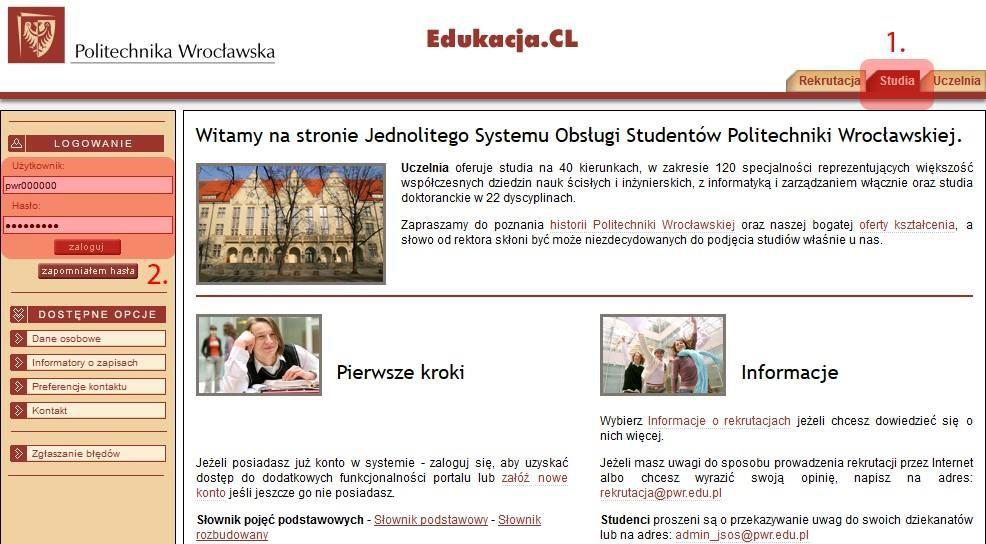
\includegraphics[scale=0.55]{photo1.png}}

\vspace{0.1cm}

\indent \hspace{0.5cm} Po zalogowaniu się do portalu Edukacja CL należy:
\item Wejść w zakładkę po lewej stronie o nazwie „Wiadomości”, a następnie klikając w odpowiednią wiadomość o temacie „Przydzielenie terminu zapisów” natrafiamy na komunikat: \\

\fbox{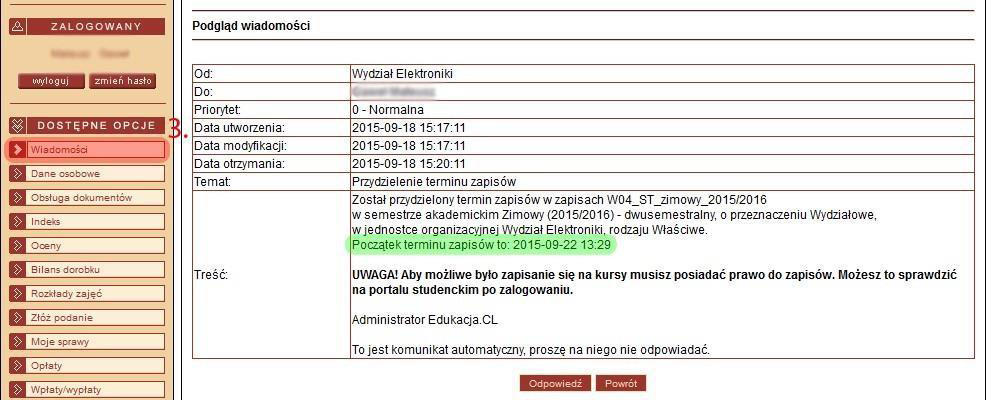
\includegraphics[scale=0.55]{photo2.png}}

\vspace{0.1cm}

\indent \hspace{0.5cm} Z wiadomości można dowiedzieć się do jakiego rodzaju zapisów termin został przydzielony, czy są to zapisy wydziałowe, ogólnouczelniane, dla jakiego wydziału oraz semestru zostały one przeznaczone, a na zielono zaznaczona jest najważniejsza informacja, a mianowicie kiedy nastąpi początek terminu zapisów. Dodatkowo w wiadomości zalecono,\linebreak by sprawdzić, czy posiadamy prawo do zapisów.\\
\indent \hspace{0.5cm} W tym celu należy po zalogowaniu się do portalu Edukacja CL:
\item Po lewej stronie wejść w zakładkę o nazwie „Zapisy”
\item Wybrać interesujący nas semestr akademicki w tabeli „Semestry” klikając w kolumnie „Rok akademicki”
\item Wybrać interesujące nas zapisy (wydziałowe lub inne) w tabeli „Zapisy w semestrze” klikając w kolumnie „Nazwa”.
\item Pod tabelą zatytułowaną „Zapisy w semestrze” kliknąć przycisk „Sprawdzenie prawa\linebreak do zapisów”, tak jak przedstawiono to poniżej:\\

\fbox{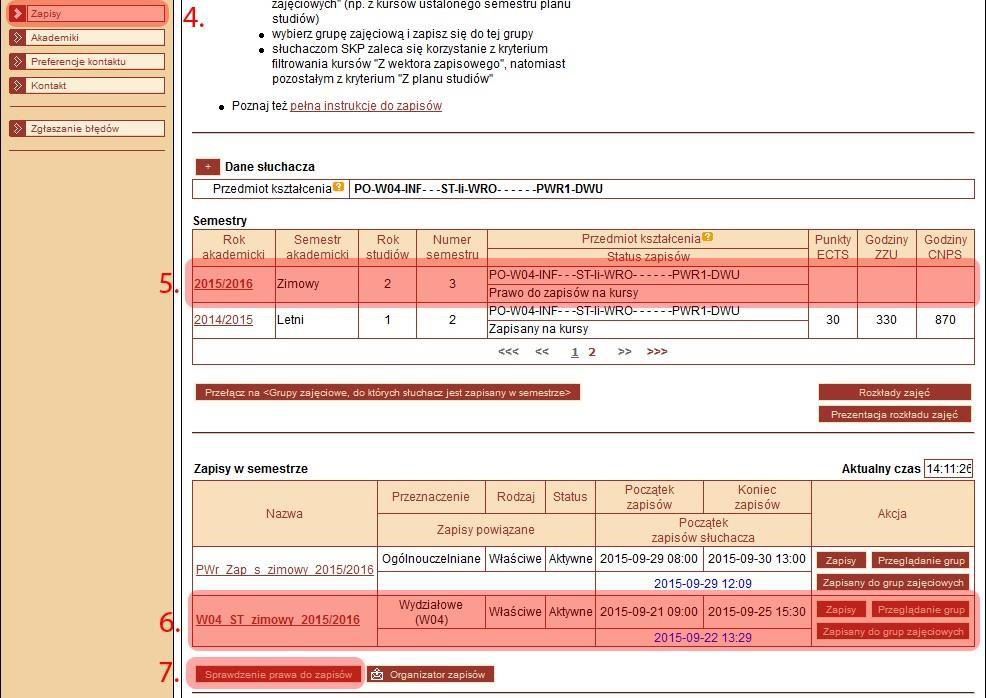
\includegraphics[scale=0.55]{photo3.png}}

\vspace{0.1cm}

Po kliknięciu otrzymujemy okno z informacją o przyznaniu prawa do zapisów:\\

\fbox{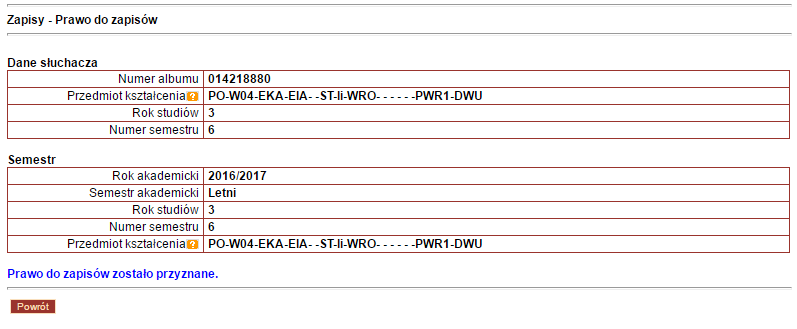
\includegraphics[scale=0.65]{photo4.png}}

\vspace{0.1cm}

\indent \hspace{0.5cm} W razie, gdyby prawo do zapisów nie zostało przyznane należy zgłosić się do sekcji informatycznej i wyjaśnić powód zaistniałej sytuacji (np. nieopłacone kursy powtórkowe, przekroczony deficyt punktowy).\\
\end{enumerate}

\subsection{WCZEŚNIEJSZE ZAPISY}
\indent \hspace{0.5cm}Na naszym wydziale istnieje możliwość złożenia wniosku o pierwszeństwo w zapisach. Wypełniony formularz dostępny na {\color{blue}{\url{http://weka.pwr.edu.pl/studenci/do-pobrania//}}} należy dostarczyć do dziekanatu przed upływem wyznaczonego terminu. 

\indent \hspace{0.5cm}Wcześniejsze zapisy wydziałowe przeznaczone są dla Studentów:
\begin{enumerate}
    \item Niepełnosprawnych
    \item Reprezentujących społeczność studencką Wydziału Elektroniki w:
        \begin{enumerate}
        \item Parlamencie Studentów Politechniki Wrocławskiej,
        \item Senacie Politechniki Wrocławskiej,
        \item Radzie Konsultacyjnej Wydziału Elektroniki,
        \item Radzie Starostów Wydziału Elektroniki jako Przewodniczący.
        \end{enumerate}
    \item Mających bardzo dobre wyniki w nauce lub/i działają aktywnie na rzecz Wydziału,
wykazujących aktywność naukową, bądź znajdujących się w szczególnej sytuacji.
\end{enumerate}
W przypadku 3. punktu Dziekan Wydziału określa całkowitą liczbę miejsc. O kolejności uzyskania prawa do wcześniejszych zapisów decyduje \textbf{suma uzyskanych punktów}. Liczone są one w następujący sposób:
\begin{center}
   \textbf{ ilość punktów = \\= średnia ważona z poprzedniego roku akademickiego x 100 + dodatkowe punkty}
\end{center}
Dodatkowe punkty przyznawane są \textbf{za działalność na rzecz Wydziału Elektroniki}, takie jak:
\begin{enumerate}[I.]
    \item Działalność w Samorządzie Studenckim (punkty przyznaje Przewodniczący) 
    \item Działalność jako Starosta (punkty przyznaje Przewodniczący Rady Starostów) 
    \item Działalność w Kole Naukowym (punkty przyznaje Opiekun Koła w porozumieniu z Przewodniczącym/Prezesem) 
    \item Inna działalność naukowa, w tym osiągnięcia uzyskane poza kołami naukowymi, (punkty przyznaje właściwy Prodziekan) zgodnie z ustaloną punktacją podaną poniżej. 
\end{enumerate}
 oraz za \textbf{działalność naukową Studentów:} 
\begin{enumerate}[I.]
    \item Konkursy
        \begin{enumerate}
            \item osiągnięcie międzynarodowe 
            \item osiągnięcie ogólnopolskie 
            \item osiągnięcie lokalne
        \end{enumerate}
    \item Szkolenia, granty, prace naukowe, warsztaty, artykuły itp. 
        \begin{enumerate}
            \item zasięg międzynarodowy 
            \item zasięg ogólnopolski 
            \item zasięg lokalny
        \end{enumerate}
\end{enumerate}
Dodatkowe punkty można uzyskać również ze względu na \textbf{działalność w komisji Samorządu Studentów Politechniki Wrocławskiej}, w tym wypadku punkty przyznaje przewodniczący danej komisji. 

\indent \hspace{0.5cm} Aby wniosek był rozpatrywany, minimalna średnia ważona ocen uzyskana w
poprzednim roku akademickim nie \textbf{może być mniejsza niż 4,00} (w przypadku gdy student może uzyskać punkty za średnią ocen). Ilość zrealizowanych punktów ECTS w poprzednim roku akademickim \textbf{nie może być mniejsza niż 40} (nie dotyczy studentów I semestru I-go i II-go stopnia). Obie te rzeczy nie oznaczają jednak, że wcześniejsze zapisy na pewno zostaną Wam przyznane. Co semestr każdy kierunek ma określony próg punktowy, który należy przekroczyć, aby otrzymać wcześniejsze zapisy. 

\textbf{1. Jak wyliczyć średnią ważoną do wniosku na konkretnych semestrach?}
\begin{figure}[H]
    \centering
    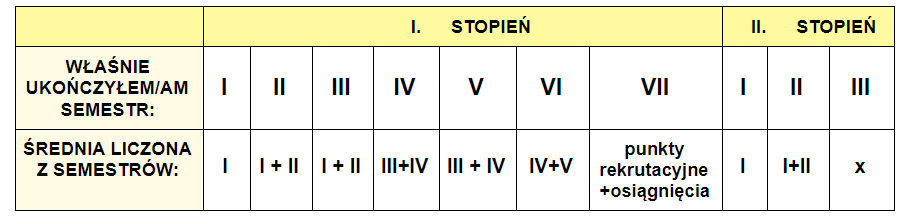
\includegraphics[width=\linewidth]{wczezapisy.png}
\end{figure}

\textbf{2. Co wpisać w rubrykę “Stopień/rok/semestr studiów”?}\\
Należy wpisać dane widoczne na {\color{blue}{\url{https://edukacja.pwr.wroc.pl/}}} w zakładce “indeks”.\\ Przykład: jeśli właśnie ukończyłeś/aś 3. semestr, musisz wpisać \textit{“1. stopień/2. rok/ 3. semestr”}.

\textbf{3. Co wpisać w rubrykę “Właściwy Prodziekan”?}\\
Tytuł naukowy oraz imię i nazwisko prodziekana ds. studenckich.\\ Na chwilę obecną jest to dr inż. Adam Wąż. 

\textbf{4. Jak wyliczyć średnią, jeśli nie zaliczyłem/am jakiegoś kursu?}\\
	Niestety niezaliczone kursy również są brane pod uwagę przy wyliczaniu średniej (w takim przypadku dodajemy ocena 2.0 x pkt. ECTS za dany kurs)  \\
	Jeśli dany kurs został poprawiony w kolejnym semestrze, również branym pod uwagę przy wyliczaniu średniej, to należy do niej dodać: $\frac{\mbox{(ocena 2.0 + nowa ocena) x pkt. ECTS za dany kurs}}{\mbox{pkt. ECTS za dany kurs x 2}} $\\(przykład: niezaliczony kurs z 1. semestru został poprawiony na 2. semestrze).\\
	Natomiast jeśli chodzi o rubrykę \textit{“Ilość zrealizowanych ECTS w poprzednim roku akademickim”} w obu przypadkach należy wpisać ilość widoczną na {\color{blue}{\url{https://edukacja.pwr.wroc.pl/}}} po ukończeniu danych semestrów w zakładce “zapisy”. \\
	
\textbf{5. Co jeśli zrealizowałem/am w danych semestrach niektóre kursy awansem? }\\
	Są one brane pod uwagę przy wyliczaniu średniej oraz przy ilości zrealizowanych ECTS tak samo jak inne kursy. Przykład: na 2 semestrze realizowałeś dodatkowo język za 3 ECTS. Jeśli zaliczyłeś wszystkie kursy, Twoja ilość zrealizowanych ECTS po dwóch semestrach wynosi 63. 
	
\textbf{6.  Co jeśli właśnie ukończyłem/am VII semestr? }\\
	W przypadku studentów rekrutujących się na 1. semestr studiów II-go stopnia przy przyznawaniu wcześniejszych zapisów brana jest pod uwagę liczba punktów rekrutacyjnych oraz obligatoryjnie odpowiednio udokumentowana działalność naukowa bądź samorządowa.
	
\textbf{7. Czy osiągnięcia sportowe pozwolą mi uzyskać dodatkowe punkty? }\\
	Niestety nie. 
	
\textbf{8. Inne ważne informacje:}
\begin{enumerate}[a)]
    \item O wcześniejsze zapisy może ubiegać się również student, który pobiera Stypendium Rektora kategorii I, lub uzyskana średnia ważona za poprzedni rok akademicki umożliwiałaby pobieranie takiego stypendium (dotyczy osób, które mogą uzyskać punkty wyłącznie z tytułu średniej ocen).
    \item Studia na drugim kierunku są brane pod uwagę, jeśli trwają dłużej niż 2 semestry.
    \item Praca zawodowa nie jest brana pod uwagę przy przydzielaniu wcześniejszych zapisów.
    \item Średnia ważona uzyskana w poprzednim roku akademickim obliczana jest z następującego wzoru: 
    \begin{equation*}
        \mbox{średnia ważona}=\frac{\sum (\mbox{ocena x punkty ECTS})}{\sum \mbox{punkty ECTS} }
    \end{equation*}
    \item W przypadku innej, poza kołem naukowym, działalności naukowej o ilości przyznanych punktów decyduje Prodziekan.
\end{enumerate}




\subsection{PLAN STUDIÓW}
\indent \hspace{0.5cm} Plan studiów zawiera listę zajęć obowiązkowych do zaliczenia, aby ukończyć studia. Znajdują się w nim informacje odnośnie tygodniowej liczby godzin przeznaczonej na zajęcia, liczby punktów ECTS (European Credit Transfer System), formy zaliczenia (tj. egzamin lub zaliczenie), liczby godzin ZZU i liczby godzin CNPS. Oznaczenia w planie studiów: w - wykład, ć - ćwiczenia, l - laboratoria, p - projekty, s – seminaria, oznaczają rodzaje odbywających\linebreak się na uczelni kursów. Plan studiów prezentuje się następująco:\\

\fbox{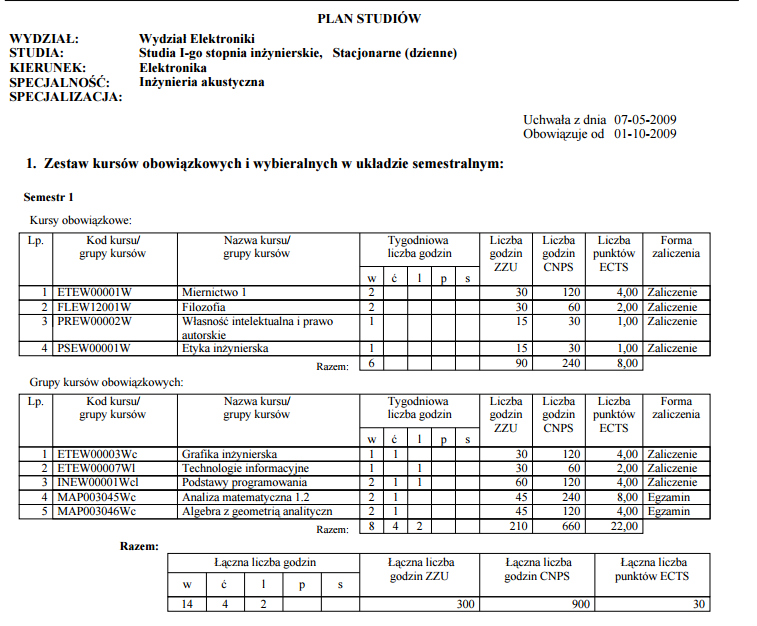
\includegraphics[scale=0.75]{photo5.png}}

\vspace{0.1cm}

Aby otworzyć plan studiów należy:
\begin{enumerate}
    \item Otworzyć w prawym górnym rogu zakładkę „Uczelnia”
    \item Otworzyć po lewej stronie zakładkę „Program nauczania/plan studiów”
    \item Z tabeli „Programy nauczania plany studiów” w kolumnie „Wydruki” kliknąć „Plan studiów”, tak jak przedstawiono to poniżej:
    
    \fbox{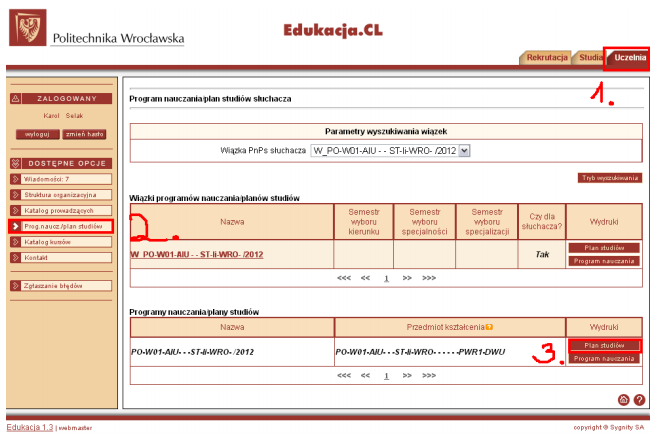
\includegraphics[scale=0.75]{photo6.png}}

\vspace{0.1cm}
\end{enumerate}
\subsection{ROZKŁAD ZAJĘĆ}
\indent \hspace{0.5cm} Znajomość rozkładu zajęć nie jest konieczna, ale może okazać się pomocna. Rozkład zajęć to tygodniowa siatka, na której widać, kiedy odbywają się dane zajęcia. Rozkładu zajęć należy szukać w serwisie „Edukacja.cl” w zakładce „Rozkłady zajęć”. Po znalezieniu odpowiedniej zakładki pobieramy plik dla interesującego nas roku na studiach o odpowiadającej mu nazwie np. „I rok”. Po otworzeniu otrzymujemy dokument, który przedstawiono poniżej (powiększenie rozkładu można znaleźć na ostatniej stronie tego dokumentu):\\

\fbox{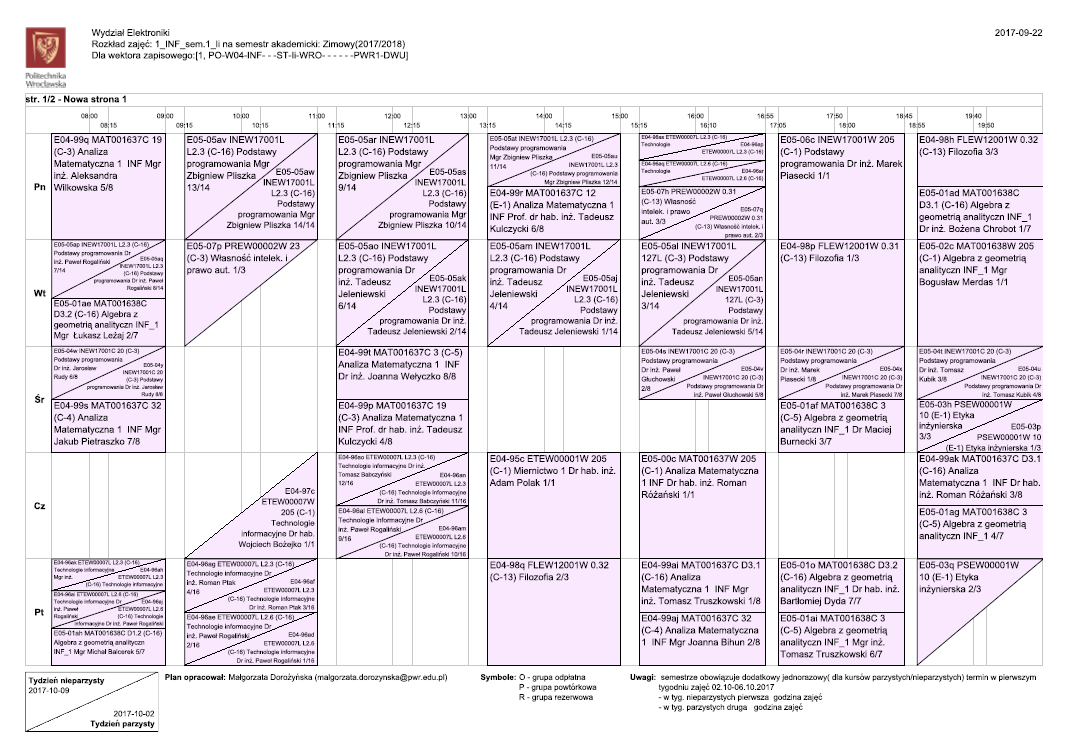
\includegraphics[scale=0.52]{photo7.png}}

\vspace{0.1cm}

Każdy z widocznych prostokątów to termin zajęć dla jednej grupy zajęciowej.\linebreak Przykładowo ćwiczenia z Analizy Matematycznej 1 to zajęcia, które mają odbywać się co tydzień i trwać 1,5 h, a w rozkładzie w tygodniu widnieje osiem takich prostokątów, czyli utworzono osiem grup. Oznacza to, że wybieramy jedną, bo każdy student może zapisać się do tylko jednej (gdzie termin go bardziej satysfakcjonuje lub w którym są nadal wolne miejsca zapisowe). Prostokąty „przekreślone” to zajęcia odbywające się co dwa tygodnie na zmianę. Górny trójkąt odpowiada zajęciom w tygodniach nieparzystych, dolny – w tygodniach parzystych. \linebreak W tego typu prostokącie są dwie grupy zajęciowe. Warto zapisać się na obie, jeśli są to dwa inne kursy, bo unikniemy przez to okienka co drugi tydzień. Litery C, P, L, S i W w dolnym narożniku oznaczają kolejno: ćwiczenia, projekt, laboratorium, seminarium oraz wykład, czyli charakter zajęć. Aby uzyskać szczegółowe informacje odnośnie zajęć, należy na portalu Edukacja CL wejść w „Przeglądanie grup”.

\subsection{PRZEGLĄDANIE GRUP}
\indent \hspace{0.5cm} Przeglądanie grup na portalu zawiera pełen zakres informacji odnośnie kursów, jednak dostęp do niego mamy tylko w określonych porach. Czas przeznaczony na przeglądanie grup możemy sprawdzić w tabeli na portalu w następujący sposób:
\begin{enumerate}
    \item Wejść w zakładkę po prawej stronie „Studia”.
    \item Po lewej stronie wejść w zakładkę „Zapisy”.
    \item Na dole strony widniej tabela zawierająca dokładny rozkład zapisów m.in. czas na przeglądanie grup, zapisy oraz czas na ewentualne poprawki.
\end{enumerate}
\indent \hspace{0.5cm} Po zapoznaniu się z planem studiów, rozkładem zajęć można przystąpić do układania własnego planu. W tym celu należy na portalu Edukacja CL:
\begin{enumerate}
    \item Wejść w zakładkę po prawej stronie „Studia”.
    \item Po lewej stronie wejść w zakładkę „Zapisy”.
    \item W tabeli „Zapisy w semestrze” w ostatniej kolumnie kliknąć „Przeglądanie grup”.
\end{enumerate}
\fbox{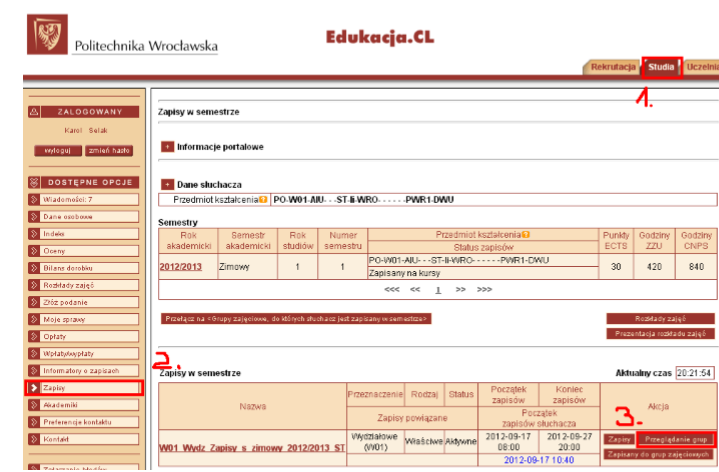
\includegraphics[scale=0.8]{photo8.png}}

\vspace{0.2cm}

\indent \hspace{0.5cm} W kolejnym oknie należy wybrać kryterium filtrowania. Mamy do dyspozycji cztery opcje:
\begin{itemize}
    \item Z planu studiów, do których słuchacz ma uprawnienia – zostaną wyświetlone wszystkie grupy zajęciowe z danego kursu (nawet te z innych kierunków na tym samym roku\linebreak i wydziale)
    \item Z wektora zapisowego, do których słuchacz ma uprawnienia – zostaną wyświetlone tylko\linebreak i wyłącznie grupy zajęć z twojego kierunku studiów
    \item Kursy powtórkowe – kursy, które są niezaliczone przez studenta
    \item Kursy zaległe – kursy, które zostały jeszcze niezrealizowane przez studenta
\end{itemize}

\fbox{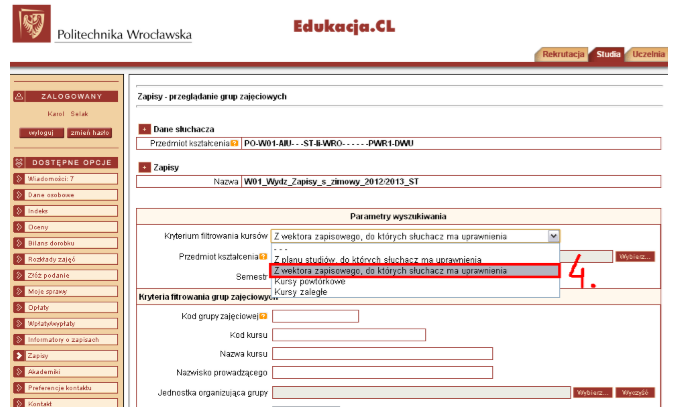
\includegraphics[scale=0.85]{photo9.png}}

\vspace{0.2cm}

\indent \hspace{0.5cm} W celu przeglądania grup kursów najlepiej wybierać kryterium: „Z wektora zapisowego, do których słuchacz ma uprawnienia”. Mamy wtedy pewność, że nie będziemy mieć żadnych problemów z potokami itd. Czasem zdarzają się sytuację, że nie możemy zapisać się na kurs\linebreak z naszego wektora zapisowego (nakładające się zajęcia, brak miejsc, itp.), wtedy używamy zapisów z planu. Po wybraniu kryterium otrzymujemy okno z tabelą, w której znajdują się nazwy\linebreak i kody kursów, na które musimy się zapisać, tak jak pokazano to poniżej:

\vspace{0.2cm}

\fbox{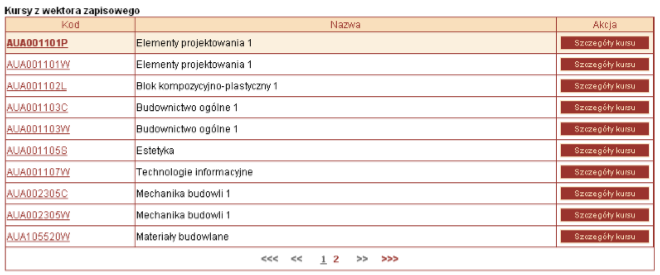
\includegraphics[scale=0.85]{photo10.png}}

\vspace{0.1cm}

\indent \hspace{0.5cm} Po wybraniu danego kursu wyświetli się lista dostępnych grup. Wybieramy tę, którą jesteśmy zainteresowani (możemy zasięgnąć rady starszych kolegów i koleżanek lub skorzystać z forum). Dalej włączamy dowolny program do gromadzenia danych
(najwygodniejszy jest Excel) i kopiujemy sobie kod upatrzonej grupy, który oznaczony jest poniżej na kolor czerwony.\linebreak Tak samo robimy z resztą kursów.

\fbox{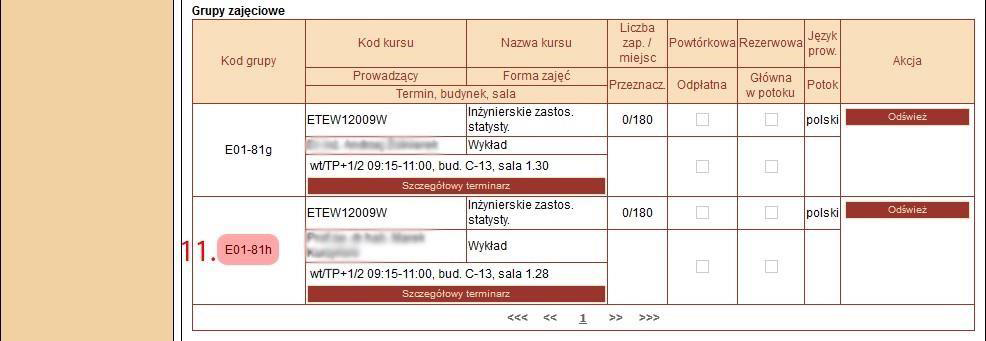
\includegraphics[scale=0.55]{photo11.png}}

\vspace{0.1cm}

\indent \hspace{0.5cm} Podczas zapisów ważne abyś zwrócił uwagę na to by:
\begin{itemize}
    \item zajęcia nie nakładały się ze sobą (z wyjątkiem tych odbywających się co dwa tygodnie,\linebreak czyli na zmianę. Grupy tę można poznać po oznaczeniu „TP”, „TN” oraz „+1/2” w rubryce zawierającej termin. Na Politechnice Wrocławskiej obowiązuje podział tygodni ze względu na parzystość „TP” – tydzień parzysty oraz „TN” – tydzień nieparzysty.\linebreak Zajęcia tę odbywają się co dwa tygodnie. Oznaczenie „+1/2” odnosi się do tygodnia „wyrównawczego”, który występuje raz na początku semestru. Przez pierwszy tydzień semestru odbywają się wszystkie zajęcia zarówno z tygodnia parzystego i nieparzystego. Zajęcia, które odbywają się co tydzień trwają tyle ile w planie (przykładowo 2 h), natomiast zajęcia odbywające się w tygodnie parzyste trwają przez pierwsze 60 min, a zajęcia z tygodnia nieparzystego przez kolejne 60 min);
    \item unikać przechodzenia z jednego budynku do drugiego w jednym dniu (np. trzeba uważać, jeśli zapiszecie się na zajęcia, które odbywają się na głównym kampusie i na Wydziale Architektury, ponieważ Wydział Architektury jest oddalony od głównego kampusu\linebreak o 10-15 minut pieszo);
    \item zaznaczyć sobie tylko po jednej grupie z każdego kursu, który Cię obowiązuje;
    \item nie mieszać potoków (jeśli jakiś kurs składa się z grupy kursów np. z wykładu i ćwiczeń, aby mieć pewność, że zapiszemy się do grupy ćwiczeniowej, która będzie realizować zajęcia zgodnie z założeniami wykładu musimy wybrać ten sam potok). Sprawdzić z jakiego potoku jest wykład lub ćwiczenia możemy w kolumnie „Potok” (typ potoku oznaczony\linebreak na czerwono), tak jak przedstawiono to poniżej:
\end{itemize}

\fbox{
\includegraphics[scale=0.55]{photo12.png}}

\vspace{0.1cm}

\indent \hspace{0.5cm} Aby wybrać ćwiczenia, które będą odpowiednie dla naszego wykładu, musimy poszukać ćwiczeń z taką samą nazwą potoku jak wykład. Tak, jak przedstawiono to poniżej:\\

\fbox{
\includegraphics[scale=0.55]{photo13.png}}

\vspace{0.1cm}

\indent \hspace{0.5cm} Gdy ułożysz swój wymarzony plan, będziesz mieć pewność, że spełniłeś wszystkie powyższe wskazówki oraz spisałeś listę kodów swoich grup (co jest szczególnie ważne, gdyż przed swoim terminem zapisowym w danym dniu nie masz dostępu do przeglądania grup zajęciowych) to możesz przystąpić do zapisów.

\subsection{ZAPISY}
\indent \hspace{0.5cm} Najpierw otwórz swój dokument z kodami grup zajęciowych. Logujemy się do naszego konta na portalu Edukacja CL. Następnie, gdy nastanie już czas naszych zapisów:
\begin{enumerate}
    \item Klikamy w prawym górnym rogu w zakładkę „Studia”.
    \item Klikamy po lewej stronie w zakładkę „Zapisy”.
    \item W tabeli „Zapisy w semestrze” w ostatniej kolumnie „Akcja” klikamy na przycisk „Zapisy”.
\end{enumerate}

\fbox{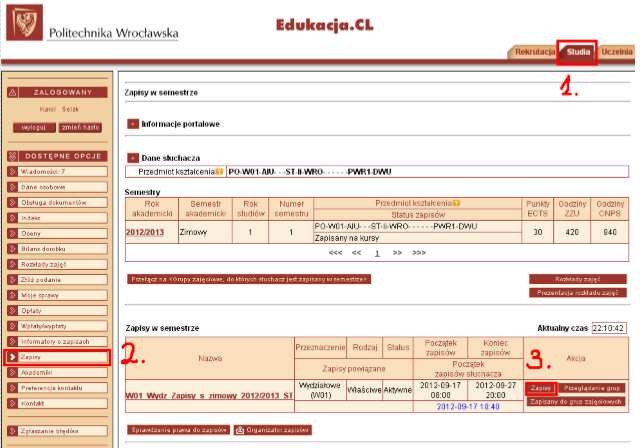
\includegraphics[scale=0.85]{photo14.png}}

\vspace{0.1cm}

\indent \hspace{0.5cm} Po tym uruchomi się formularz zapisowy, jak poniżej. Do okienka wpisujemy po kolei kody grup z Excela. Po każdej akceptując klikając „Zapisz”.

\fbox{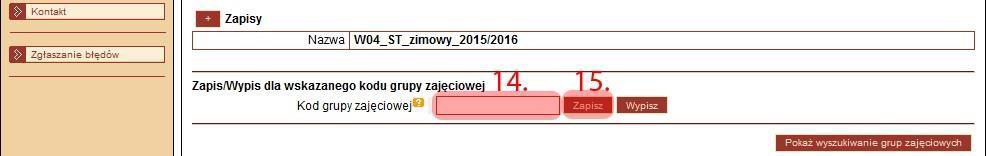
\includegraphics[scale=0.55]{photo15.png}}

\vspace{0.1cm}

\indent \hspace{0.5cm} W razie pomyłki lub chęci zamiany grupy istnieje możliwość wypisania się z danego kursu, poprzez kliknięcie przycisku „Wypisz”. Każdy swój błąd masz szansę naprawić, dopóki trwają zapisy oraz w trakcie korekt. Jeśli wszystko poszło dobrze podczas zapisu do grupy powinien pokazać się komunikat:

\fbox{
\includegraphics[scale=0.55]{photo16.png}}

\vspace{0.1cm}

\indent \hspace{0.5cm} Oprócz komunikatu z powodzeniem możemy otrzymać różne komunikaty z błędami. \linebreak Przy pierwszych zapisach najczęstsze z nich to:
\begin{itemize}
    \item brak miejsca w grupie zajęciowej,
    \item niezgodność potoku grupy wykładowej z formami towarzyszącymi (ćwiczenia, laboratoria, itp.), próba zapisu na kurs, na który już wcześniej się zapisaliśmy.
\end{itemize}

\indent \hspace{0.5cm} W obu przypadkach musimy wybrać inny kurs, w którym są wolne miejsca\linebreak lub który będzie zgadzać się z potokiem wybranym podczas zapisów na inne zajęcia z grupy kursów.\\

\indent \hspace{0.5cm} Jeśli poprawnie zapisaliśmy się na wszystkie kursy to powinniśmy otrzymać łączną liczbę punktów ZZU, CNPS, ECTS tak jak w naszym planie studiów na dany semestr.\\

\indent \hspace{0.5cm} Powodzenia!
\newpage

\fbox{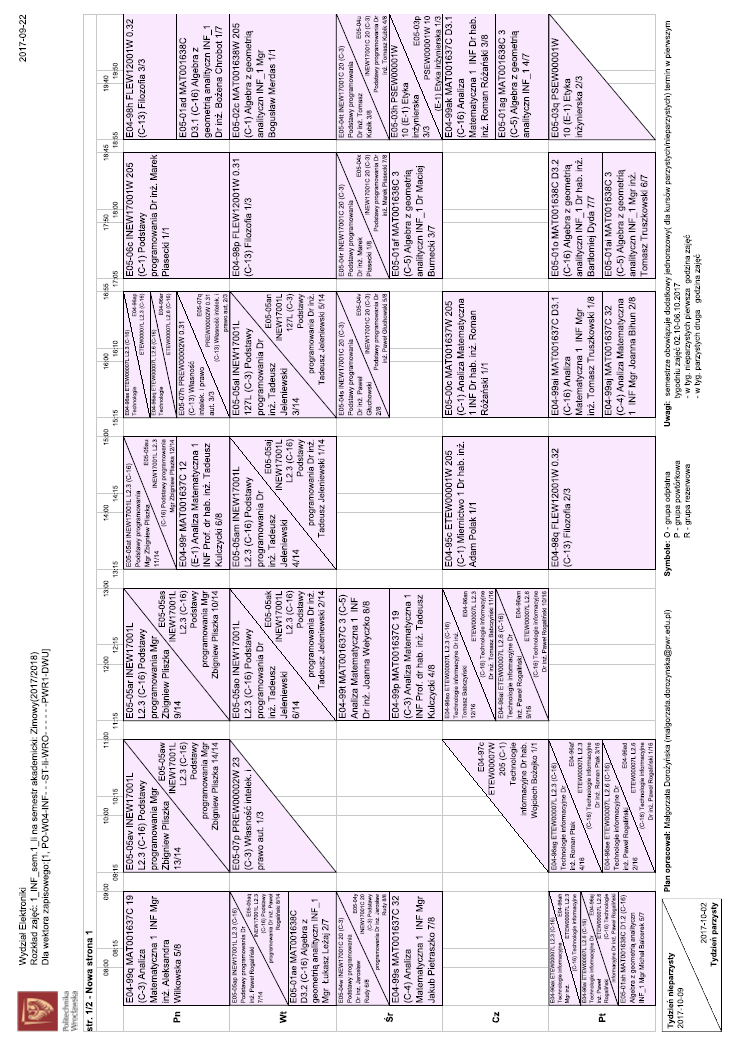
\includegraphics[scale=0.8]{photo17.png}}

\end{document}